\documentclass{sig-alternate-05-2015}
\usepackage[utf8]{inputenc}
\usepackage[italian]{babel}
\usepackage[T1]{fontenc}
\usepackage{graphicx}
\usepackage{graphics}
\usepackage{listings}  
\usepackage{array}
\newcolumntype{L}[1]{>{\raggedright\let\newline\\\arraybackslash\hspace{0pt}}m{#1}}
\newcolumntype{C}[1]{>{\centering\let\newline\\\arraybackslash\hspace{0pt}}m{#1}}
\newcolumntype{R}[1]{>{\raggedleft\let\newline\\\arraybackslash\hspace{0pt}}m{#1}}
\usepackage{multirow}
\usepackage[table]{xcolor}
\usepackage{float}
\usepackage{array}
\usepackage{ragged2e}
\usepackage{cleveref}
\newcolumntype{P}[1]{>{\RaggedRight\hspace{0pt}}p{#1}}

\lstset{language=Java,tabsize=2,basicstyle=\ttfamily\scriptsize} 

\newcommand{\squeezeup}{\vspace{-0.5mm}}

\usepackage{etoolbox}
\makeatletter
\patchcmd{\@makecaption}
{\scshape}
{}
{}
{}
\makeatother

\newcolumntype{"}{@{\hskip\tabcolsep\vrule width 1pt\hskip\tabcolsep}}

\lstdefinestyle{base}{
	language=C,
	emptylines=1,
	breaklines=true,
	basicstyle=\ttfamily\color{black},
	moredelim=**[is][\color{red}]{@}{@},
}

\newcommand\FIXME[1]{\textbf{FIXME: #1}}

\begin{document}

% Copyright
\setcopyright{acmcopyright}
%\setcopyright{acmlicensed}
%\setcopyright{rightsretained}
%\setcopyright{usgov}
%\setcopyright{usgovmixed}
%\setcopyright{cagov}
%\setcopyright{cagovmixed}


%% DOI
%\doi{10.475/123_4}

%% ISBN
%\isbn{123-4567-24-567/08/06}

%Conference
\conferenceinfo{MSR '17}{May 20--21, 2017, Buenos Aires, Argentina}

%\acmPrice{\$15.00}

%
% --- Author Metadata here ---
%\conferenceinfo{WOODSTOCK}{'97 El Paso, Texas USA}
%\CopyrightYear{2007} % Allows default copyright year (20XX) to be over-ridden - IF NEED BE.
%\crdata{0-12345-67-8/90/01}  % Allows default copyright data (0-89791-88-6/97/05) to be over-ridden - IF NEED BE.
% --- End of Author Metadata ---

\title{Are We Reusing Outdated Code from Stack Overflow?}

\numberofauthors{1}
\author{
	\alignauthor
	$^1$Chaiyong Ragkhitwetsagul, $^1$Jens Krinke, $^2$Giuseppe Bianco \\
	\affaddr{$^1$University College London, London, UK}\\
	\affaddr{$^2$Università degli Studi del Molise, Campobasso, Italy}
}


\maketitle
\begin{abstract}
This paper provides a sample of a \LaTeX\ document which conforms,
somewhat loosely, to the formatting guidelines for
ACM SIG Proceedings. It is an {\em alternate} style which produces
a {\em tighter-looking} paper and was designed in response to
concerns expressed, by authors, over page-budgets.
It complements the document \textit{Author's (Alternate) Guide to
Preparing ACM SIG Proceedings Using \LaTeX$2_\epsilon$\ and Bib\TeX}.
This source file has been written with the intention of being
compiled under \LaTeX$2_\epsilon$\ and BibTeX.

The developers have tried to include every imaginable sort
of ``bells and whistles", such as a subtitle, footnotes on
title, subtitle and authors, as well as in the text, and
every optional component (e.g. Acknowledgments, Additional
Authors, Appendices), not to mention examples of
equations, theorems, tables and figures.

To make best use of this sample document, run it through \LaTeX\
and BibTeX, and compare this source code with the printed
output produced by the dvi file. A compiled PDF version
is available on the web page to help you with the
`look and feel'.
\end{abstract}

\section{Introduction}
%The popularity of the Internet encourages tremendous amount of source code being shared online. 
Stack Overflow is a popular online programming community with 6.3 million users. It allows programmers to ask questions and give answers to programming problems. The website has found to be useful for software development and also valuable for educational purposes \cite{x}. On Stack Overflow, each conversation contains a question and answer(s).  The answers normally contain at least one code snippet as a solution to the question asked. The code snippet is usually not written directly on Stack Overflow website but copied from another location. It can be copied and modified from the problematic code snippet in the question, copied from an answerer's own code, or borrowed from other locations including open source software (OSS) systems. As a result, the process of posting and answering questions on Stack Overflow which involves copying and pasting source code can be considered as code cloning. 

Code cloning is an activity of reusing source code by copying and pasting. It normally occurs in software development and account from 7\% to 23\% in typical software systems \cite{Bellon2007}. The benefits and drawbacks of clones are still controversial. Several authors state that clones lead to bug propagations and software maintenance issues \cite{Kamiya2002}, while some others have proofs that in some cases clones are not harmful than normal code or even beneficial \cite{Saini2016,Kapser2006}. Code cloning can also have side effects of violating software licenses. Carelessly cloning code from one project and reusing it in another project with different license may cause software licensing violation \cite{German2009}.

In this study, we treat code snippets that are copied from software systems to Stack Overflow, and vice versa, as code clones. We call them \textbf{online code clones}. There are three ways to create online code clones: 1) code is cloned from a software project to Stack Overflow as an example; 2) code is cloned from Stack Overflow to a software project to obtain a functionality, perform a particular task, or fixing a bug; and 3) code is implicitly cloned from one software project to another by having Stack Overflow as a medium. Online code clones can similarly lead to a problem of bug propagation as classical code clones. Unfortunately, they are more difficult to locate and fix since the search space from online corpora is larger and no longer confined in a local repository.

A motivating example of problems caused by online code clones can be found in a Stack Overflow post regarding how to implement RawComparator in Hadoop\footnote{http://stackoverflow.com/questions/22262310}. In \Cref{fig:before-after}, the left hand side shows a code snippet embedded as a part of accepted answer to the question. The snippet shows how Hadoop implements \textit{compare} method in its \textit{WritableComparator} class. The code snippet on the right hand side shows another version of the same \textit{compare} method in \textit{WritableComparator} class but it is extracted from the latest version of Hadoop. We can obviously see that they are highly similar except one line, \verb|buffer.reset(null,0,0);|, added in the latest version after \verb|key2.readFields(buffer);|. The added line is intended for cleaning up the reference in \verb|buffer| variable. While this change has already been introduced into \textit{compare} method in the latest version of Hadoop, the code example in Stack Overflow post is still unchanged and outdated. This example shows that there can be inconsistencies between online code clones and its original.  %Since reusing source code from Stack Overflow is considered a common practice nowadays, the scale of online code cloning is more than intra or inter project clone in a local code bases. 
This is an emerging and challenging problem. Since studies in this area are still limited, we aim to gain more insight of the problem in this study. %We are interested to gain more insights of online code clone in this study.

\begin{figure*}
\begin{lstlisting}
/* Code in Stack Overflow #22315734 */                      /* WritableComparator.java (2016-09-26) */
1 public int compare (byte[] b1,int s1,int l1,              1 public int compare(byte[] b1,int s1,int l1,
2                     byte[] b2,int s2,int l2) {            2                    byte[] b2,int s2,int l2) {
3   try {                                                   3   try {
4     buffer.reset(b1,s1,l1); /* parse key1 */              4     buffer.reset(b1,s1,l1); /* parse key1 */
5     key1.readFields(buffer);                              5     key1.readFields(buffer);
6     buffer.reset(b2,s2,l2); /* parse key2 */              6     buffer.reset(b2,s2,l2); /* parse key2 */
7     key2.readFields(buffer);                              7     key2.readFields(buffer);
8   } catch (IOException e) {                               8     buffer.reset(null,0,0); /* clean up reference */
9     throw new RuntimeException(e);                        9   } catch (IOException e) {
10   }                                                      10    throw new RuntimeException(e);
11   return compare(key1,key2); /* compare them */          11  }
12 }                                                        12  return compare(key1, key2); /* compare them */
                                                            13 }
\end{lstlisting}
\caption{The same code fragments, WritableComparator.java, on Stack Overflow post 22315734 and latest version in hadoop code base}
\label{fig:before-after}
\end{figure*}

This paper makes the following  primary contributions:

\vspace{0.5ex}%
\noindent\textbf{1.~A manual study of online code clones:} 
We used two clone detection tools to discover 266,837,480 similar code fragment pairs and manually investigated 7,840 candidate clone pairs between Java code fragments obtained from Stack Overflow accepted answers and 109 Java open source projects.

\vspace{0.5ex}%
\noindent\textbf{2.~Addressing the problems of reusing source code between open source projects and Stack Overflow:} Our study shows that there are at least 84 clones that have been obviously copied from open source projects to Stack Overflow as code examples which potentially violate their software licenses. Furthermore, 50 out of the 84 clones are outdated and questionable for being reused.

\section{Empirical Study}
We perform an empirical study of online code clones between Stack Overflow and 109 Java open source projects to answer the following research questions: \\ 
\textbf{RQ1 (online code clones):} \textit{To what extent  source code is cloned between Stack Overflow and open source projects?} We would like to quantitatively measure the number of online code clones between Stack Overflow and open source projects to understand the scale of the problem. \newline
%\textbf{RQ2 (flow of online code clones):} \textit{what are the directions that source code is cloned?} If clones between the two locations exist, we would like to observe in which direction the code has been copied. Is it mostly from Stack Overflow to open source projects, or the other way around, or equally both? \newline
\textbf{RQ2 (classification of online code clones):} \textit{What are the main characteristics among the set of online code clones?} We group them into seven groups according to our pre-defined classification scheme so we can differentiate and understand the motivation of cloning. Some of the clones are copy from open source projects to Stack Overflow, while some are copied from a third-party location, and some are accidental clones containing boiler-plate code, and code stubs generated by IDE. \newline
\textbf{RQ3 (effects of online code clones):} \textit{what are the effects derived from online code clones? can they be harmful to software development?} Is there observable problems caused by clones between Stack Overflow and open source projects?

\begin{figure*}
	\centering
	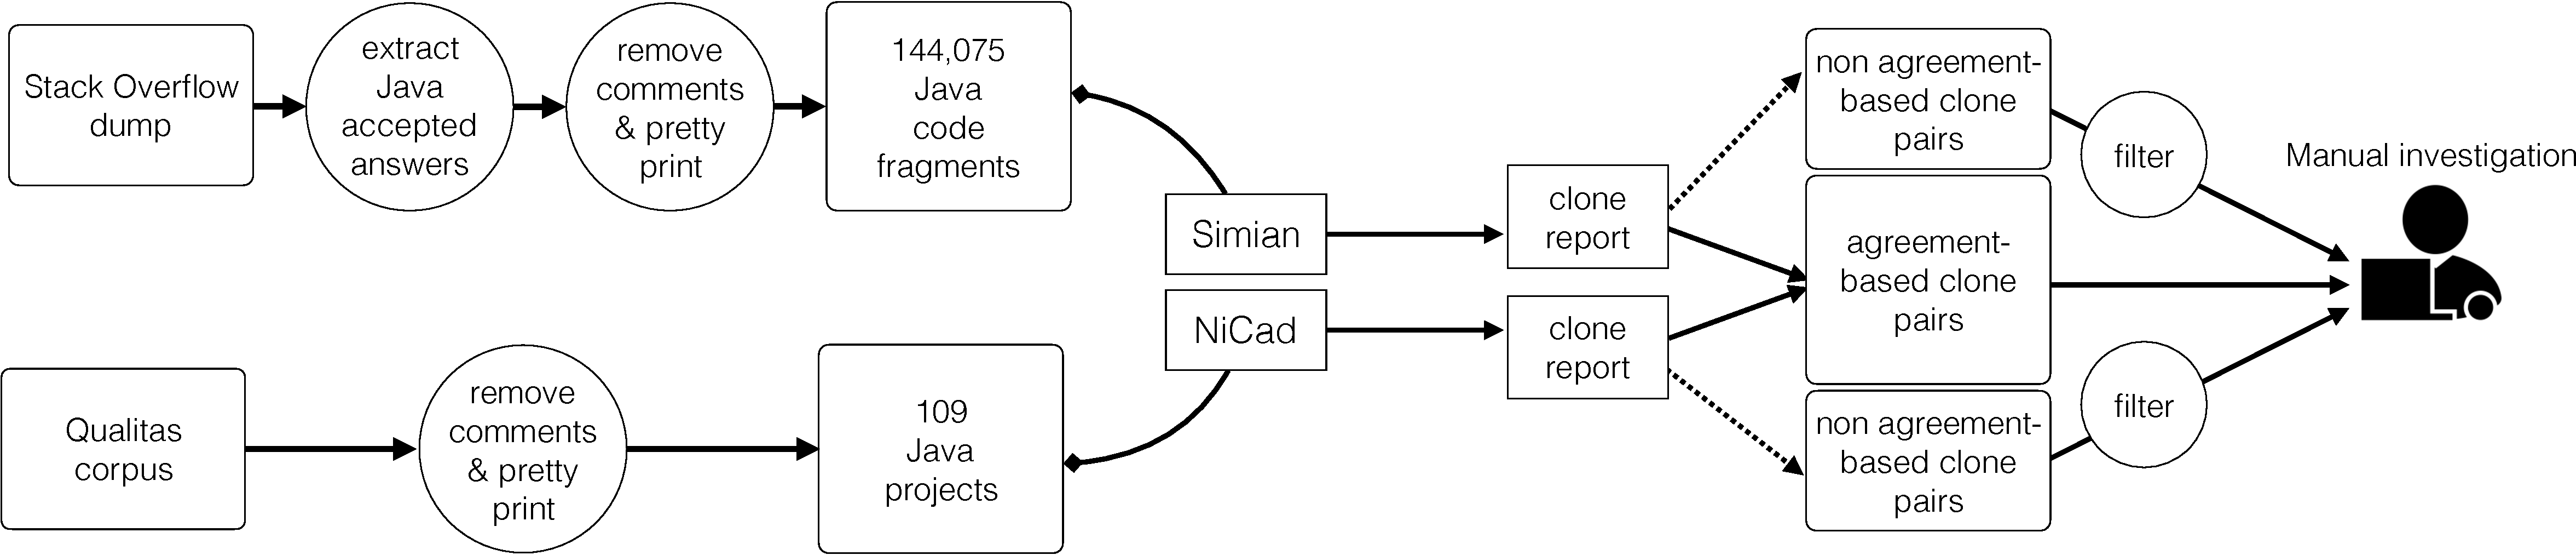
\includegraphics[width=0.9\linewidth]{exp_framework}
	\caption{Experimental framework}
	\label{fig:exp_framework}
\end{figure*}

\subsection{Experimental Framework}
To answer the three research questions, an experimental framework is designed as depicted in \Cref{fig:exp_framework}. We process two datasets, Stack Overflow and open source projects from Qualitas corpus. Java code fragments are extracted from Stack Overflow posts using regular expressions. We pre-process Java code in both datasets by removing comments and pretty-printing to increase accuracy of clone detection. Then, we deploy two clone detection tools, Simian \cite{simian} and NiCad \cite{Roy2008,Cordy}, to locate clones between the two datasets. Due to a technical limit of Simian and NiCad to scale to large datasets, we partition the input and run the tools multiple times. Each run is composed of the whole Stack Overflow data and a single Qualitas project. We repeat the process until we cover 109 projects. 

We then convert the clone reports to General Clone Format (GCF)~\cite{Wang2013} and combine them into a single file. GCF provides a common format for clones which enable us to reuse scripts that analyse clone reports from Simian and NiCad. Moreover, using GCF, other additional clone detectors can be adopted, if needed, without any changes in the analysis. Simian do not provide an option to detect inter clones between two locations. Hence the Simian GCF clone report is pruned to contain only inter clone pairs between Stack Overflow and Qualitas project. In this step, all intra clone pairs within Stack Overflow and open source projects are removed. NiCad provides an option to detect inter clones so no pruning is needed. Next, clone pairs reported from the two clone detectors are pair-wise matched to find agreements using Bellon's clone overlapping criteria \cite{Bellon2007}. This step generates \textbf{agreement-based clone pairs}. They are clones with highest confidence since they receive agreement from both tools. Then, clone pairs reported by Simian and NiCad that do not find agreement are filtered by size of minimum 10 lines. This step generates \textbf{non agreement-based clone pairs}. The non agreement-based clone pairs are clones with less confidence than agreement-based ones. Finally, agreement-based and non agreement-based clone pairs are looked at and classified manually by the first author.

In the manual inspection process, we classify clones into categories according to their properties. This process takes approximately a months until we successfully classified 7,840 clone pairs into categories. Some of the clone candidates are false clones due to being boiler-plate code or IDE-generated and are discarded for further analysis. By ignoring the false clones, we compare licensing information of x,xxx remaining clone pairs for possibility of software licensing violations. Moreover, we look forward through history of the clones from the projects' git versioning systems. This is to see if there is any changes made to the clones after it has been copied, hence resulting in outdated clones on Stack Overflow.

\subsection{Experimental Setup}

\subsubsection{Datasets}
\begin{table}
	\centering
	\caption{Stack Overflow and Qualitas datasets}
	\label{tab:datasets}
	\small
	\begin{tabular}{l|r|r}
		\hline 
		Dataset & No. of files & SLOC \\
		\hline
		Stack Overflow & 144,075 & 2,347,269 \\ 
		\hline 
		Qualitas &  138,238 & 16,081,899 \\ 
		\hline 
	\end{tabular} 
\end{table}

\textbf{Stack Overflow}: we extracted Java code snippets from accepted answers in a snapshot of Stack Overflow dump \footnote{https://archive.org/details/stackexchange} in January 2016. The archived dump has a size of 9 gigabytes. The data dump is in XML format containing information of \textit{Posts} (questions and answers) and supporting data such as user accounts and timestamps of the posts. We are interested in code snippets embedded in posts which are pieces of code located between \texttt{<code></code>} tags. We filtered the snippets with two filtering criteria. First, we ignore snippets that are less than 6 lines since they are usually not considered as clones by clone detection research \cite{something}. Second, we are only interested in code snippets from posts that are marked accepted answer since they have high chances to be reused than snippets in questions and other answers. Each snippet is extracted from the dump using regular expressions and saved to a file using its post ID as the file's name. We use \texttt{.java} extension so that the clone detectors can recognise them. If a Stack Overflow conversation has more than one code snippet in the accepted answer, we append an indexing number starting from zero after the post ID (e.g. 45051109\_0.java, and 45051109\_1.java). With the two filters, we finally obtained 144,075 Java code snippets which contain xxx lines of Java source code excluding comments and blank lines\footnote{measured by cloc: https://github.com/AlDanial/cloc}.

\textbf{Qualitas corpus}: we selected an established corpus for empirical software engineering studies called Qualitas \cite{QualitasCorpus}. \FIXME{more details about Qualitas and why we chose it}. We selected the 20130901r version of Qualitas corpus containing 112 Java open source projects with releases no later than 1st September 2013. We chose the snapshot in 2013 since we are interested in online code clones from old releases of the software. Out of 112 Qualitas projects, there are 3 projects, \textit{eclipse}, \textit{jre}, and \textit{squirrel-sql}, that do not contain source code so they were removed from the study. This results in totally 109 projects analysed in the study. As shown in \Cref{tab:datasets}, the 109 Qualitas project have 138,238 Java files containing 16,081,899 lines of code. %Details of the 109 Qualitas projects and their licenses are listed in Table \ref{t:new_and_old}.

\subsubsection{Clone Detectors}
There are certain restrictions in terms of choosing clone detection tools for this study. Firstly, they have to compatible with Java. Secondly, due to nature of code snippets posted on Stack Overflow, some of them are not complete Java classes or methods. Hence, the tool must be flexible enough to process code snippets which are not in a complete block or not compilable. Thirdly, since the amount of code that have to be process are in a scale of millions line of source code (as shown in \Cref{tab:datasets}), a clone detector must be scalable enough to be able to successfully complete the execution and report clones in a reasonable amount of time. These restrictions force us to remove three well-known clone detectors; CCFinder \cite{Kamiya2002}, iClones \cite{Gode2009}, and DECKARD \cite{Jiang2007a}; from our study since they failed to detect clones between 144,075 Stack Overflow code snippets and 109 Qualitas projects. We finally selected two clone detectors for this study: \textbf{Simian} \cite{simian} and \textbf{NiCad} \cite{Cordy,Roy2008}. We found that both of them are flexible enough to handle million-SLOC code corpus with method or class incompleteness.

Simian is a text-based clone detector which locate clones at line-level granularity and has been used extensively in several clone studies \cite{Ragkhitwetsagul2016, Wang2013, Mondal2011, Cheung2015, Krinke2010}. It is a command-line tool which enables us to automate the detection. It also offers normalisation of variable names and literals (strings, and numbers) which enable Simian to detect clones of type 1 and type 2. NiCad is also a text-based clone detector which detects clones at method or code block granularity. It can detect clone up to type 3 and is used in several clone studies \cite{Roy2008, Ragkhitwetsagul2016, Svajlenko2014, Wang2013, Mondal2011, Sajnani2016}. It utilises TXL for parsing and pretty-printing source code. It also provide code normalisation by variable renaming and abstractions. We use a variant of NiCad called \textit{nicadcross}. It offers the same functionalities as the original NiCad but is specialised for detecting code clones between two systems.

\subsubsection{Agreement-based Clone Detection}
Since we do not have clone oracle of the two datasets, we adopted an idea of clone agreement used in clone research \cite{Wang2013,Funaro2010,cr2016ssbse} to help reducing the number of clones for manual investigation. To find agreement of two clone pairs, we resort to an approach proposed by a study by another study~\cite{Bellon2007}. 

According to Bellon et al.~\cite{Bellon2007}, \textit{good} and \textit{ok}-match clone pairs are defined as follows. A clone pair \textit{CP} is formed by two clone fragments \textit{CF$_1$} and \textit{CF$_2$} with a pre-defined similarity threshold \textit{t}: \textit{CP} = (\textit{CF$_1$}, \textit{CF$_2$}, \textit{t}). For each clone pair, we can define \textit{overlap} and \textit{contained} value of two clone pairs as 
\squeezeup
\begin{multline}
	overlap(CP_1, CP_2) = \frac{|lines(CF_1) \cap lines(CF_2)|}{|lines(CF_1) \cup lines(CF_2)|} 
\end{multline}
\squeezeup
\begin{multline}
	contained(CP_1, CP_2) = \frac{|lines(CF_1) \cap lines(CF_2)|}{|lines(CF_1)|}. 
\end{multline}

\textit{good-value} is then defined as
\squeezeup
\begin{align*}
	good(CP_1, CP_2) = min(overlap(CP_1.CF_1,CP_2.CF_1), \\ overlap(CP_1.CF_2,CP_2.CF_2)).
\end{align*}

And \textit{ok-value} is defined as
\squeezeup
\begin{align*}
	ok(CP_1,CP_2) = min(max(contained(CP_1.CF_1,CP_2.CF_1), \\ contained(CP_2.CF_1,CP_1.CF_1)),
	\\ max(contained(CP_1.CF_2,CP_2.CF_2), \\contained(CP_2.CF_2,CP_1.CF_2))).
\end{align*}

Two clone pairs $CP_1$ and $CP_2$ are called a \textit{good-match(p)} iff, for $p \in [0,1]$ holds 
\squeezeup
\begin{equation}
good(CP_1,CP_2) \geq p.
\end{equation}

Similarly for \textit{ok-match(p)} pair
\squeezeup
\begin{equation}
ok(CP_1,CP_2) \geq p.
\end{equation}

Using this \textit{good-match} and \textit{ok-match} criteria, we can prioritise clone pairs for manual investigation. \textit{good-match} pairs are the ones with the highest confident to be true clones followed by \textit{ok-match} pairs. After finishing agreement-based clone pairs, the clone pairs without agreement with be manually looked at.

\section{Results}

We are aware of effects of configurations to clone detection results and needs for searching for optimised configurations. However, considering the size of the two datasets and search space of the Simian's and NiCad's parameters, we are hindered from finding the best configurations of the tools. Thus, we decided to configure Simian and NiCad using two established settings: 1) the tools' default settings (denoted as \textit{df}), and 2) settings from \textit{EvaClone}, a study of optimising clone detectors' configurations based on clone agreement, by Wang et al.~\cite{Wang2013} (denoted by \textit{EvCl}). With two tools and two sets of configurations, we look for agreements in four pair-wise combinations: Simian$_{df}$-NiCad$_{df}$, Simian$_{df}$-NiCad$_{EvCl}$, Simian$_{EvCl}$-NiCad$_{df}$, and Simian$_{EvCl}$-NiCad$_{EvCl}$.

The clone statistics obtained from running Simian and NiCad with \textit{df} and \textit{EvCl} setting are presented in \Cref{tab:raw_stats}. Preliminary manual investigation of Simian's clone report showed that there were problematic 11 fragments. These fragments make Simian generating a large number of false clones involving array initialisation. Hence, they were removed from Simian's clone reports before the analysis. From \Cref{tab:raw_stats}, Simian clones are from approximately 10\% of the full 144,075 Stack Overflow fragments, 1,406 reported by Simain$_{df}$ and 1,360 from Simain$_{EvCl}$ respectively. NiCad$_{df}$ reports clones from 1,197 Stack Overflow fragments while NiCad$_{EvCl}$ reports clones from a large amount of 12,884 fragments due to its relaxed settings. In terms of number of clone pairs, EvaClone configurations prefer recall \cite{Wang2013} so Simian$_{EvCl}$ and NiCad$_{EvCl}$ report a large number of clone pairs of 59,936,722 and 206,718,663 respectively. The average clone size of Simian$_{df}$ is 7.45 which is bigger than the EvaClone counterpart of 4.81. Similarly, NiCad$_{df}$ has an average clone size of 9.54 which is also bigger than 5.31 reported by NiCad$_{EvCl}$. The statistics show that EvaClone tunes the tools in the way that they report smaller clones but result in higher agreements. The percentage of clone size compared to the size of Stack Overflow snippets reported by Simian$_{df}$, Simian$_{EvCl}$, NiCad$_{df}$, and NiCad$_{EvCl}$ is 28\%, 29\%, 25\% and 21\% accordingly.

\begin{table}[H]
	\centering
	\caption{No.~of projects in Qualitas successfully analysed by Simian and NiCad}
	\label{tab:projects_missing}
	\small
	\begin{tabular}{l|r|r|r|r}
		\hline
		%		\multicolumn{3}{c|}{Qualitas-\textit{O}} & \multicolumn{3}{c}{Qualitas-\textit{N}} \\
		%		\hline
		& Simian$_{\textrm{\textit{df}}}$ & Simian$_{\textrm{\textit{EvCl}}}$  & NiCad$_{\textrm{\textit{df}}}$ & NiCad$_{\textrm{\textit{EvCl}}}$ \\ % & Simian$_{\textrm{\textit{df/EvaClone}}}$ & NiCad$_{\textrm{\textit{df}}}$ & NiCad$_{\textrm{\textit{EvCl}}}$ \\ \hline
		\hline
		\textit{Successful} & 109 & 109 & 97 & 82 \\ %& 44 & 40 & 34 \\
		\textit{Clust.~fail} & -- & -- & 6 & 16 \\
		\textit{Renm.~fail} & -- &  -- & -- & 11 \\
		\hline
	\end{tabular}
\end{table}

\begin{table*}[h]
	\centering
	\caption{Statistics of clones found between Stack Overflow and Qualitas projects using Simian and NiCad}
	\label{tab:raw_stats}
%	\resizebox{\columnwidth}{!}{%
	\small
		\begin{tabular}{l|r|r|r|r|r|r|r|r|r|r|r|r}
			\hline
			\multirow{3}{*}{Statistics} 
			& \multicolumn{3}{c|}{Simian$_{df}$} 
			& \multicolumn{3}{c|}{Simian$_{\textrm{\textit{EvCl}}}$}
			& \multicolumn{3}{c|}{NiCad$_{df}$} 
			& \multicolumn{3}{c}{NiCad$_{\textrm{\textit{EvCl}}}$} \\ \cline{2-13} 
			& \multicolumn{3}{c|}{1406 fragments} 
			& \multicolumn{3}{c|}{1360 fragments}  
			& \multicolumn{3}{c|}{1197 fragments} 
			& \multicolumn{3}{c}{12884 fragments} \\ \cline{2-13}
			%& \multicolumn{3}{c|}{iCharC,iCurlB,iIdC,iMod,iStrC} 
			%& \multicolumn{3}{c|}{iCurlB,iId,iIdC,iStr,iChar,iSbtNm,bSqBrck} 
			%& \multicolumn{3}{c|}{rename=none,abstract=none} 
			%& \multicolumn{3}{c}{rename=blind,abstract=literal} \\ %\cline{2-17}  
			& $C_{\mathrm{pairs}}$ & $C_{\mathrm{SLOC}}$ & $C_{\mathrm{\%}}$ 
			& $C_{\mathrm{pairs}}$ & $C_{\mathrm{SLOC}}$ & $C_{\mathrm{\%}}$ 
			& $C_{\mathrm{pairs}}$ & $C_{\mathrm{SLOC}}$ & $C_{\mathrm{\%}}$
			& $C_{\mathrm{pairs}}$ & $C_{\mathrm{SLOC}}$ & $C_{\mathrm{\%}}$ \\ 
			\hline
			%Removed & 11 & -- & -- & -- & 0 & -- & -- & -- & -- & -- & -- & -- & -- & -- & -- & -- \\ %& 11 & -- & -- & -- \\
			Total & 54790 & -- & -- 		& 59936722 & --	& -- 		& 127305 	& -- & -- 	& 206718663 & -- & -- \\
			Mean & 52 & 7.45 & 28\% 		& 44104 & 4.81 & 29\% 		& 106 & 9.54 & 25\% 	& 16046 & 5.31 & 21\% \\
			Std Dev. & 147 & 3.22 & 23\% 	& 1040483 & 1.20 & 19\% 	& 209 & 3.10 & 18\% 	& 21890 & 1.92 & 16\% \\
			Max  & 1020 & 49.00 & 94\% 		& 38223637 & 18.00 & 89\% 	& 2100 & 39.00 & 81\% 	& 442655 & 50.00 & 93\% \\
			Min  & 1 & 5.00 & 1\% 			& 1 & 4.00 & 2\% 			& 1 & 7.00 & 2\% 		& 1 & 3.00 & 1\% \\
			Median  & 3 & 7.00 & 21\% 		& 24 & 5.00 & 25\% 			& 20 & 8.00 & 19\% 		& 8003 & 5.00 & 16\% \\
			Mode  & 1 & 7.00 & 33\% 		& 1 & 4.00 & 50\% 			& 1 & 8.00 & 67\% 		& 1 & 4.00 & 33\% \\
			\hline
		\end{tabular} %
%	}
\end{table*}

%\begin{table*}
%	\centering
%	\caption{109 Qualitas projects (new versions retrieved on 2016-09-27)}
%	\label{t:new_and_old}
%%	\resizebox{\columnwidth}{!}{%
%	\small
%		\begin{tabular}{l|r|r|c|c|p{3cm}|p{3cm}}
%			\hline 
%			Projects & Old version & New versions & Latest change & CVS & License & Notes \\
%			\hline
%			antlr4 & 4.0 & 4.5.4 & 25/09/2016 & git & BSD & \\
%			apache-ant & 1.8.4 & 1.10.0 & 09/04/2016 & git & Apache2.0 & \\
%			argouml & 0.34 & 0.35.4 & 11/01/2015 	& svn & Eclipse  1.0 & \\
%			artofillusion & 2.8.1 & 3.0.2 & 27/08/2016 & svn & GPL 2.0 & \\
%			aspectj & 1.6.9 & 1.8.9 & 12/05/2016 & git & Eclipse   1.0 & \\
%			axion & 1.0-M2 & - & 08/03/2013 & - & Proprietary (BSD/Apache-style) & \\
%			batik & 1.7 & 1.9.0 & 11/05/2016 & svn & Apache , v.2.0 & \\
%			c-jdbc & 2.0.2 & - & 16/09/2005 & - & GLGPL 2.1 & \\
%			castor & 1.3.1 & 1.4.2 & 17/08/2016 & git & Apache 2.0 & \\
%			cayenne & 3.0.1 & 4.0.M4 &  26/09/2016 & git & Apache 2.0 & \\
%			checkstyle & 5.1 & 7.2  & 23/09/2016 & git & GLGPL 2.1 \& Apache 2.0 & \textit{Cli, Logging and Beanutils} packages are from the Apache Commons project. \\
%			cobertura & 1.9.4.1 & 2.1.2 & 01/06/2016 & git & GPL 2.0  & \\
%			colt & 1.2.0 & - & 09/09/2014 & - & Proprietary (CERN) & Found multithreaded v. \\
%			columba & 1.4 & - & 20/04/2007 & - & Mozilla   1.1  & \\
%			commons-collections & 3.2.1 & 4.2 & 12/09/2016 & svn & Apache 2.0 & \\
%			compiere & 330 & - & - & - & GPL 2.0 & No longer OSS \\
%			db-derby & 10.6.1.0 & 10.12.1 & 13/08/2016 & svn & Apache 2.0 & \\
%			displaytag & 1.2 & 2.0 & 17/08/2014 & svn & MIT  & \\
%			drawswf & 1.2.9 & - & 02/04/2013 & - & GPL 2.0 & \\
%			drjava & 20100913-r5387 & ??? & 03/09/2014 & svn & BSD  & Build to see version? \\
%			exoportal & ??? & ??? &  & git & GLGPL 3.0 \& proprietary & Too many new projects \\
%			emma & 2.0.5312 & 2.0.5312 & 09/05/2013  & - & Common   1.0 & \\
%			findbugs & 1.3.9 & 3.0.1 & 06/03/2015 & - & GLGPL 2.0 & \\
%			fit-java & 1.1 & - & 04/06/2013 & - & GPL 2.0 & \\
%			fitlibrary & 20100806 & ??? & 29/07/2014 & git & GPL 2.0 & \\
%			freecol & 0.10.7 & 0.11.6 & 26/09/2016 & git & GPL 2.0 &  \\
%			freecs & 1.3.20100406 & - & 22/04/2013 & - & GPL 3.0 &   \\
%			freemind & 0.9.0 & 1.0.0 & 16/08/2016 & git & GPL 2.0+ &  \\
%			galleon & 2.3.0 & 2.5.6 & 29/04/2013 & - & GPL 2.0 & \\
%			ganttproject & 2.0.9 & 2.8.1 & 16/08/2016 & git & GPL 3.0 &  \\
%			geotools & 2.7-M3 & 16 & 27/09/2016 & git & GLGPL 2.0 & \\
%			hadoop & 1.0.0 & 3.0.0-alpha2 & 26/09/2016 & git & Apache 2.0 & \\
%			heritrix & 1.14.4 & - & 05/06/2013 & - & GLGPL 2.1 & \\
%			hibernate & 4.2.2 & 5.2.3 & 22/09/2016 & git & GLGPL 2.1+ & \\
%			hsqldb & 2.0.0 & 2.3.4 & 13/09/2016 & svn & BSD  & \\
%			htmlunit & 2.8 & 2.24 & 26/09/2016 & svn & Apache 2.0 & \\
%			ireport & 3.7.5 & - & 28/05/2014 & - & Affero GLGPL 3.0 & \\
%			itext & 5.0.3 & 5.5.9 & 27/09/2016 & git & Affero GLGPL 3.0 & \\
%			informa & 0.7.0-alpha2 & - & 07/11/2008 & - & GLGPL 2.1 \& Apache Software 1.1 & \\
%			ivatagroupware & 0.11.3 & - & 27/02/2013 & - & GPL 2.0 & \\
%			jfin\_datemath & R1\_0\_1 & - & 25/04/2013 & - & GPL 2.0 & \\
%			joggplayer & 114s & - &  15/04/2013 & - & GPL 2.0 & \\
%			jag & 6.1 & 6.2 & 08/04/2013  & - & GPL 2.0 \& BSD  & BSD  is for libraries. \\
%			james & 2.2.0 & 2.3.2.1 & 14/08/2015 & - & Apache 2.0 & \\
%			jasml & 0.10 & - & 08/03/2013 & - & Apache Software  & \\
%			jasperreports & 3.7.4 & 6.3.1 & 27/09/2016 & git & GLGPL 3.0 &  \\
%			javacc & 5.0.0 & 7.0.0 & 15/08/2016 & svn & Proprietary (Sun) & \\
%			jboss (wildfly) & 5.1.0.GA & 11.0.0.Alpha1 & 27/09/2016 & git & GLGPL 2.1 & Renamed to Wildfly. \\
%			jchempaint & 3.0.1 & 3.4 & 01/09/2016 & git & GLGPL 2.1+ &  \\
%			jedit & 4.3.2 & 5.3.1 & 20/09/2016 & svn & GPL 2.0 &  \\
%			jena & 2.6.3 & 3.1.1 & 16/09/2016 & git & Apache 2.0 & \\
%			jext & 5.0 & - & 18/08/2004 & - & GPL 2.0 &  \\
%			jfreechart & 1.0.13 & 1.5.0 & 29/08/2016 & git & GLGPL 2.0 &   \\
%			jgraph & 5.13.0.0 & 3.6.0.0 & 07/09/2016 & git & Proprietary (mxGraph) & \\
%			jgraphpad & 5.10.0.2 & - & 10/11/2006 & - & GPL   \& GLGPL (derivatives) & \\
%			jgrapht & 0.8.1 & 1.0.1 & 23/09/2016 & git & GLGPL 2.1 \& Eclipse  1.0 & \\
%			jgroups & 2.10.0.GA & 4.0.0 & 26/09/2016 & git & Apache 2.0 & \\
%			jmoney & 0.4.4 & ??? & 27/12/2015 & git & GPL 2.0 &  \\
%			jparse & 0.96 & - & 29/07/2004 & - & GLGPL 2.1 & \\
%			jpf & 1.5.1 & ??? & 13/01/2012 & - & Apache 2.0 & \\
%			junit & 4.11 & 4.12 & 04/12/2014 & git & Eclipse  1.0 & \\
%			shiftone-jrat & 0.6 & 1-beta-1 & 17/11/2007 & svn & GLGPL 2.0 &  \\
%			vuze & 4812 & 5730 & 23/09/2016 & svn & GPL 2.0 & \\
%			\hline
%		\end{tabular} %
%%	}
%\end{table*}

\begin{table}
	\centering
	\caption{13 Qualitas projects that have been cloned as examples on Stack Overflow}
	\label{t:new_and_old}
	%	\resizebox{\columnwidth}{!}{%
	\small
	\begin{tabular}{l|r|p{3.5cm}}
		\hline 
		Project & Version & License  \\
		\hline
%		apache-ant & 1.8.4 & Apache2.0 \\
%		apache-log4j & 1.2.16 & \\
		apache-tomcat & 7.0.2 & \\
		aspectj & 1.6.9 & Eclipse 1.0 \\
		hadoop & 1.0.0 & Apache 2.0\\
		hibernate & 4.2.2 & GLGPL 2.1+ \\
		jasperreports & 3.7.4 & GLGPL 3.0  \\
		jfreechart & 1.0.13 & GLGPL 2.0  \\
		jgraph & 5.13.0.0 & Proprietary (mxGraph) \\
%		jgrapht & 0.8.1 & GLGPL 2.1 \& Eclipse  1.0 \\
		jstock & 1.0.7c & \\
		jung2 & 2\_0\_1 & \\
		junit & 4.11 & Eclipse  1.0 \\
		poi & 3.6 & \\
		spring-framework & 3.0.5 & \\
		struts2 & 2.2.1-all & \\
%		weka & 3-7-9 & \\
		\hline
	\end{tabular} %
	%	}
\end{table}
			
%\begin{table*}
%	\centering
%	\caption{109 Qualitas projects (new versions retrieved on 2016-09-27)}
%	\label{t:new_and_old}
%	%	\resizebox{\columnwidth}{!}{%
%	\small
%	\begin{tabular}{l|r|r|c|c|p{3cm}|p{3cm}}
%		\hline 
%			Projects & Old version & New versions & Latest change & CVS & License & Notes \\
%			\hline
%			apache-jmeter & 2. 9 & & & & & \\
%			apache-log4j & 1.2.16 & & & & & \\
%			apache-maven & 3.0 & & & & & \\
%			apache-roller & 4.0.1 & & & & & \\
%			apache-tomcat & 7.0.2 & & & & & \\
%			jhotdraw & 7.5.1 & & & & & \\
%			jrefactory & 2.9.19 & & & & & \\
%			jruby & 1.5.2 & & & & & \\
%			jspwiki & 2.8.4 & & & & & \\
%			jstock & 1.0.7c & & & & & \\
%			jsxe & 04\_beta & & & & & \\
%			jtopen & 7\_1 & & & & & \\
%			jung2 & 2\_0\_1 & & & & & \\
%			lucene & 4.3.0 & & & & & \\
%			marauroa & 3.8.1 & & & & & \\
%			megamek & 0.35.18 & & & & & \\
%			mvnforum (mvnad) & 1.2.2 (1.0.1) & & & & & \\
%			myfaces-core & 2.0.2 & & & & & \\
%			nakedobjects & 4.0.0 & & & & & \\
%			nekohtml & 1.9.14 & & & & & \\
%			netbeans & 6.9.1 & & & & & \\
%			openjms & 0.7.7-beta-1 & & & & & \\
%			oscache & 2.4.1 & & & & & \\
%			picocontainer & 2.10.2 & & & & & \\
%			pmd & 4.2.5 & & & & & \\
%			poi & 3.6 & & & & & \\
%			pooka & 080505 & & & & & \\
%			proguard & 4.5.1 & & & & & \\
%			quartz & 1.8.3 & & & & & \\
%			quickserver & 1.4.7 & & & & & \\
%			quilt & 0.6-a-5 & & & & & \\
%			rssowl & 2.0.5 & & & & & \\
%			sablecc & 3.2 & & & & & \\
%			sandmark & & & & & & \\
%			spring-framework & 3.0.5 & & & & & \\
%			struts2 & 2.2.1-all & & & & & \\
%			sunflow & 0.07.2 & & & & & \\
%			tapestry & 5.1.0.5 & & & & & \\
%			trove & 2.1.0 & & & & & \\
%			velocity & 1.6.4 & & & & & \\
%			wct-package & 1.5.2 & & & & & \\
%			webmail & 0.7.10 & & & & & \\
%			weka & 3-7-9 & & & & & \\
%			xalan-j & 2\_7\_1 & & & & & \\
%			xerces-J & 2.10.0 & & & & & \\
%			xmojo & 5.0.0 & & & & & \\
%			\hline 
%		\end{tabular} %
%%	}
%\end{table*}

%\subsection{Agreement based clone pairs vs. Non agreement based clone pairs}

%The agreement-based clone pairs are the ones discovered using Bellon's \textit{good}-match(0.7) and \textit{ok}-match(0.7) criteria as listed in  Table \ref{t_agreed_good_clone_pairs}. Non-agreement based clone pairs are the ones that are solely reported by a single tool. The agreement-based pairs provide higher confident that they are real clones than the non-agreement based ones.

\subsection{Agreement based clone pairs}

We use a threshold \textit{p} of 0.7 for both \textit{good} and \textit{ok}-match. A visualisation of \textit{good}-match clone pairs between four sets of parameter settings can be seen from \Cref{fig:venn4_orig_good}. There are 2,261 unique \textit{good}-match pairs. The distribution of 23,868 \textit{ok}-match pairs, which subsume the \textit{good}-match pairs, is depicted in \Cref{fig:venn4_orig_ok}.

Nevertheless,  NiCad produced renaming and clustering errors for some of the settings. This resulted in not all 109 projects had NiCad clone reports. For NiCad default settings (NiCad$_{\textrm{\textit{df}}}$), 6 projects had clustering failed errors. For NiCad EvaClone settings (NiCad$_{\textrm{\textit{EvCl}}}$), 4 projects had renaming failed errors and 13 projects had clustering failed errors as depicted in \Cref{tab:projects_missing}. So these projects are also missing from agreed clone pairs. \FIXME{Report the errors to NiCad creator.}

%\FIXME{Maybe no longer needed?} We are interested in discovering reused code in the latest versions of Qualitas projects. So, we downloaded the newest release of each project and found 44 of them having newer updates. Then, we reran the experiment again on these 44 projects. Several projects triggered NiCad problem of clustering and renaming again as listed in Table \{tab:projects_missing}. The agreed clone pairs using Bellon's \textit{good}-match(0.7) and \textit{ok}-match(0.7) criteria of this new dataset are also listed in Table \{t_agreed_good_clone_pairs}. 

\begin{table}[H]
	\centering
	\caption{Distribution of agreement-based clone pairs using Bellon's criteria}
	\label{t_agreed_good_clone_pairs}
	\small
	\begin{tabular}{l|l|r|r}
		\hline
		\multicolumn{2}{c|}{Tool} & \multicolumn{2}{c}{No.~of clone pairs} \\
		\hline
		Simian & NiCad & \textit{good}-match & \textit{ok}-match \\
		%\hline
		%Settings & Simian$_{\mathrm{\textit{default}}}$ & Simian$_{\mathrm{\textit{EvaClone}}}$ & Simian$_{\mathrm{\textit{default}}}$ & Simian$_{\mathrm{\textit{EvaClone}}}$ \\ % & Simian$_{\mathrm{\textit{cloplag}}}$ \\
		\hline
		\textit{default} & \textit{default} & 10 	& 3800 \\ 
		\textit{default} & \textit{EvaClone} 	& 26 	& 1017 \\ 
		\textit{EvaClone} 	& \textit{default} 	& 10 	& 88 \\
		\textit{EvaClone} 	& \textit{EvaClone} 	& 2228 & 19777 \\ 
		\hline
		\multicolumn{2}{l|}{Total} & 2274 & 24682 \\
		\hline
		\multicolumn{2}{l|}{Total (unique)} & 2261 & 23868 \\
		\hline
	\end{tabular}
\end{table}

\begin{figure*}
	\begin{minipage}{.5\textwidth}
		\centering
		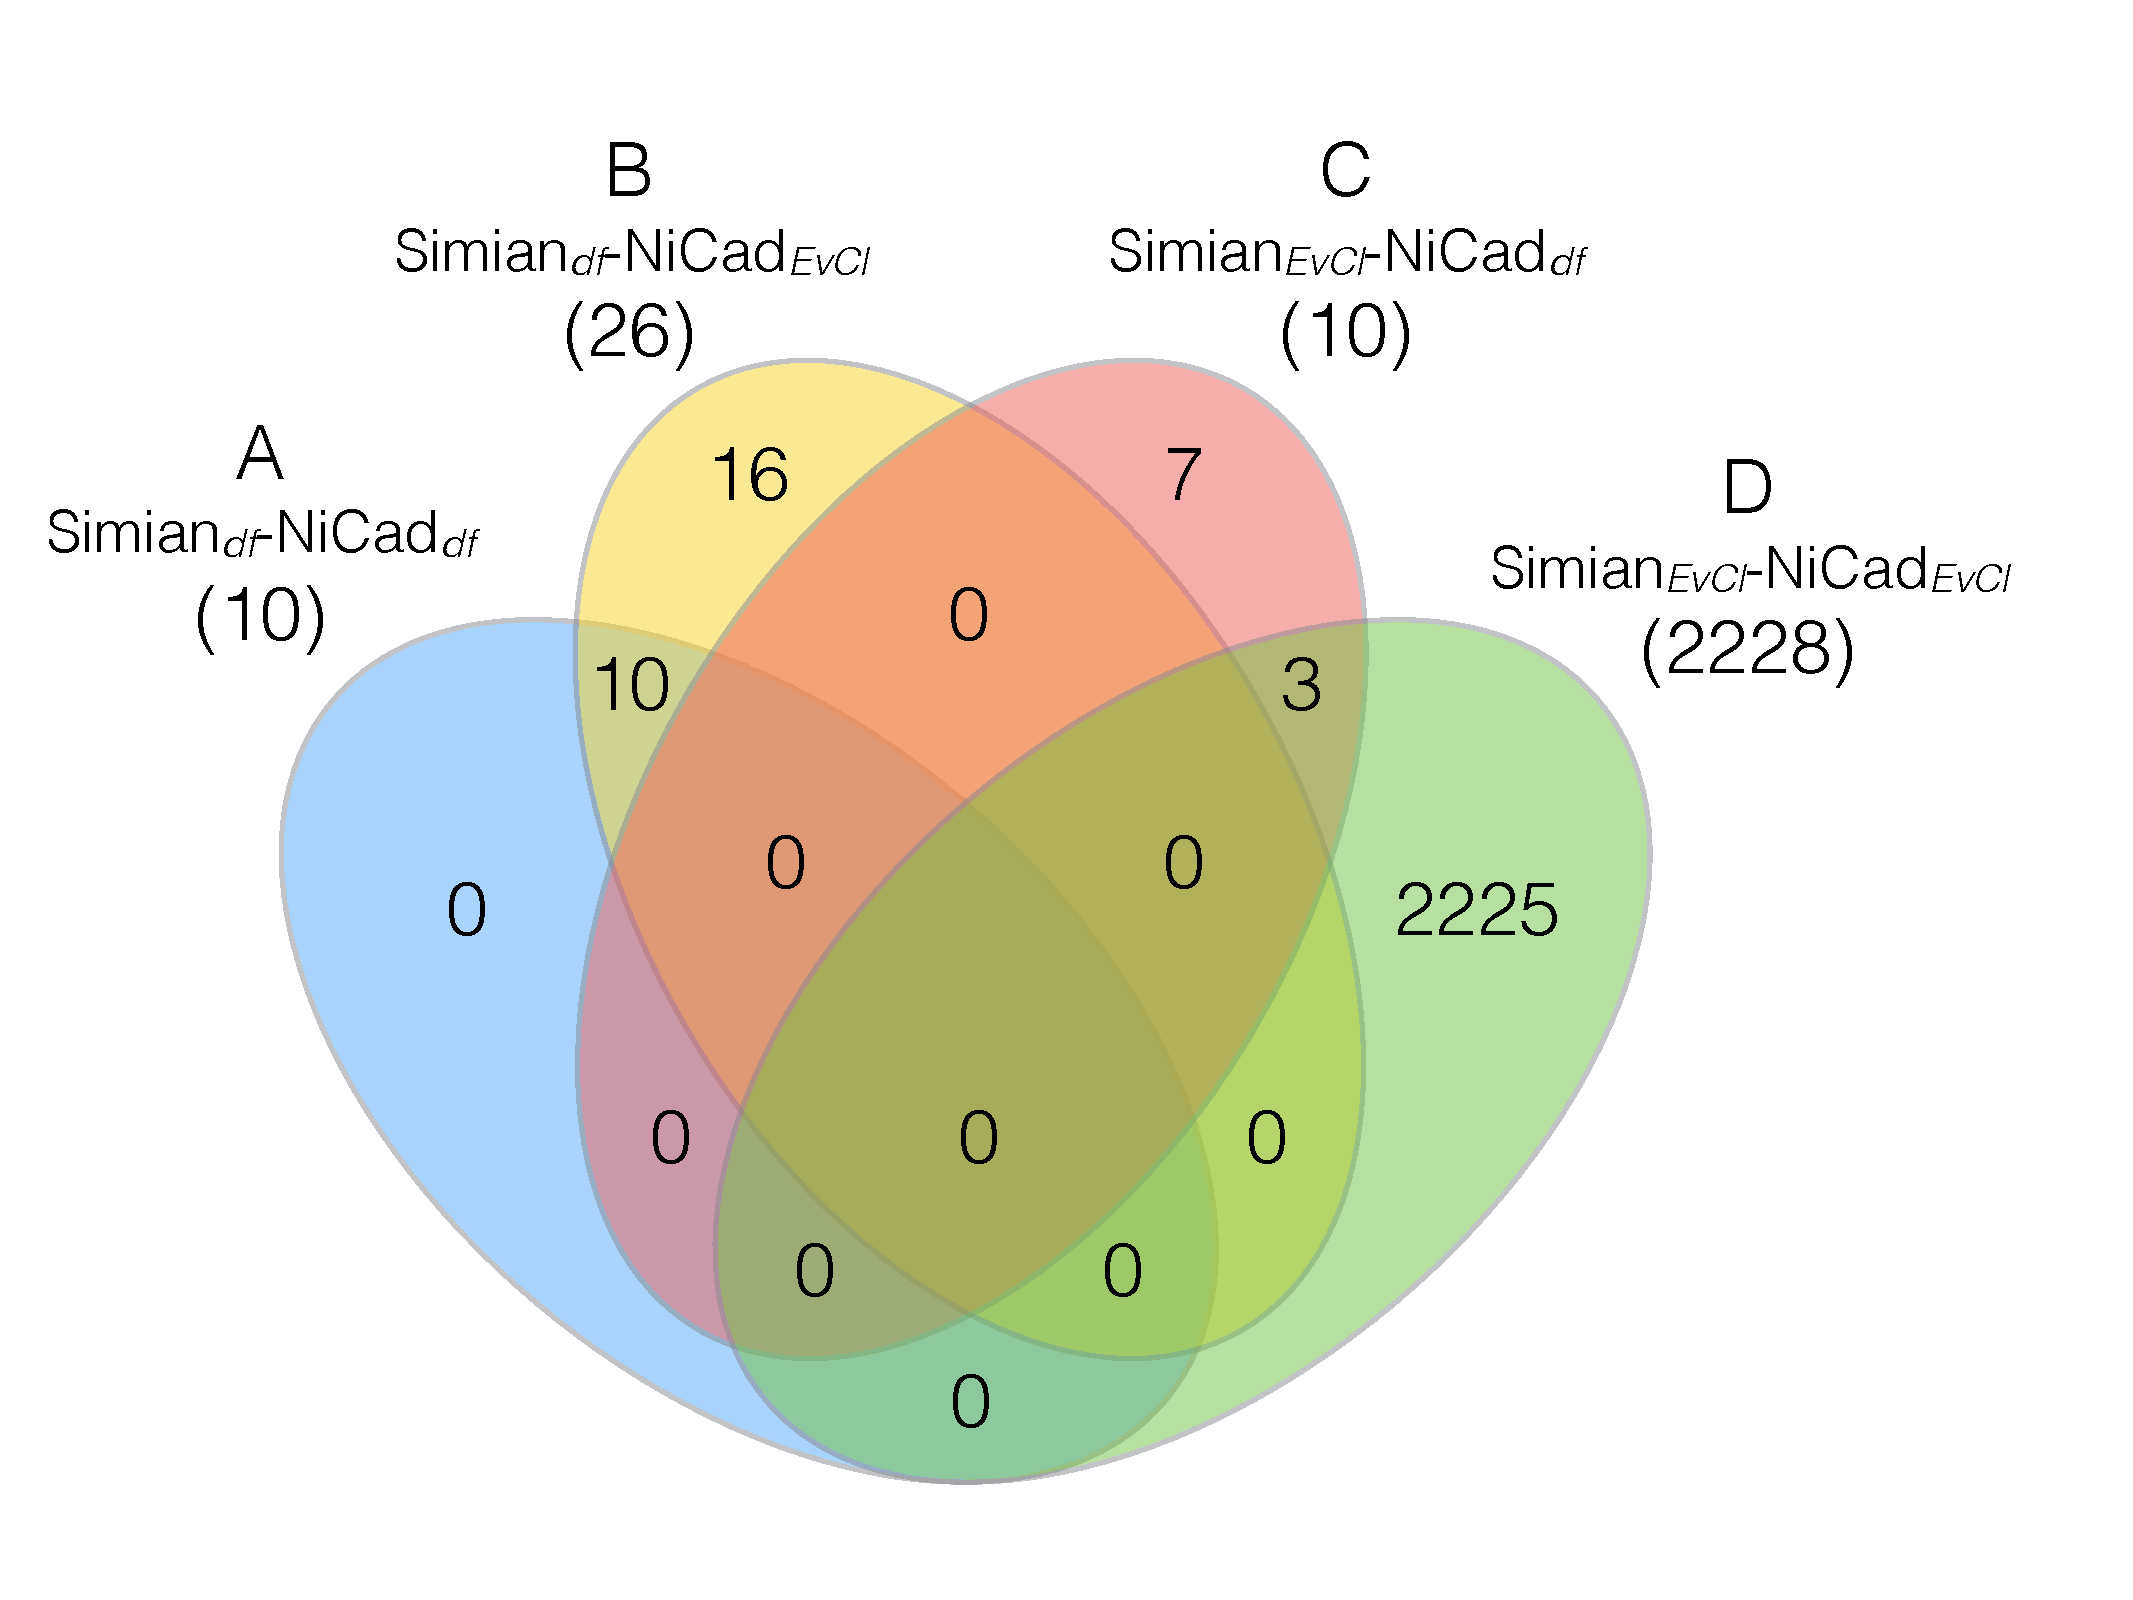
\includegraphics[width=0.8\linewidth]{venn4_pairs_good_pt1+2}
		\caption{Distributions of \textit{good}-match(0.7) pairs}
		\label{fig:venn4_orig_good}
	\end{minipage}
	\begin{minipage}{.5\textwidth}
		\centering
		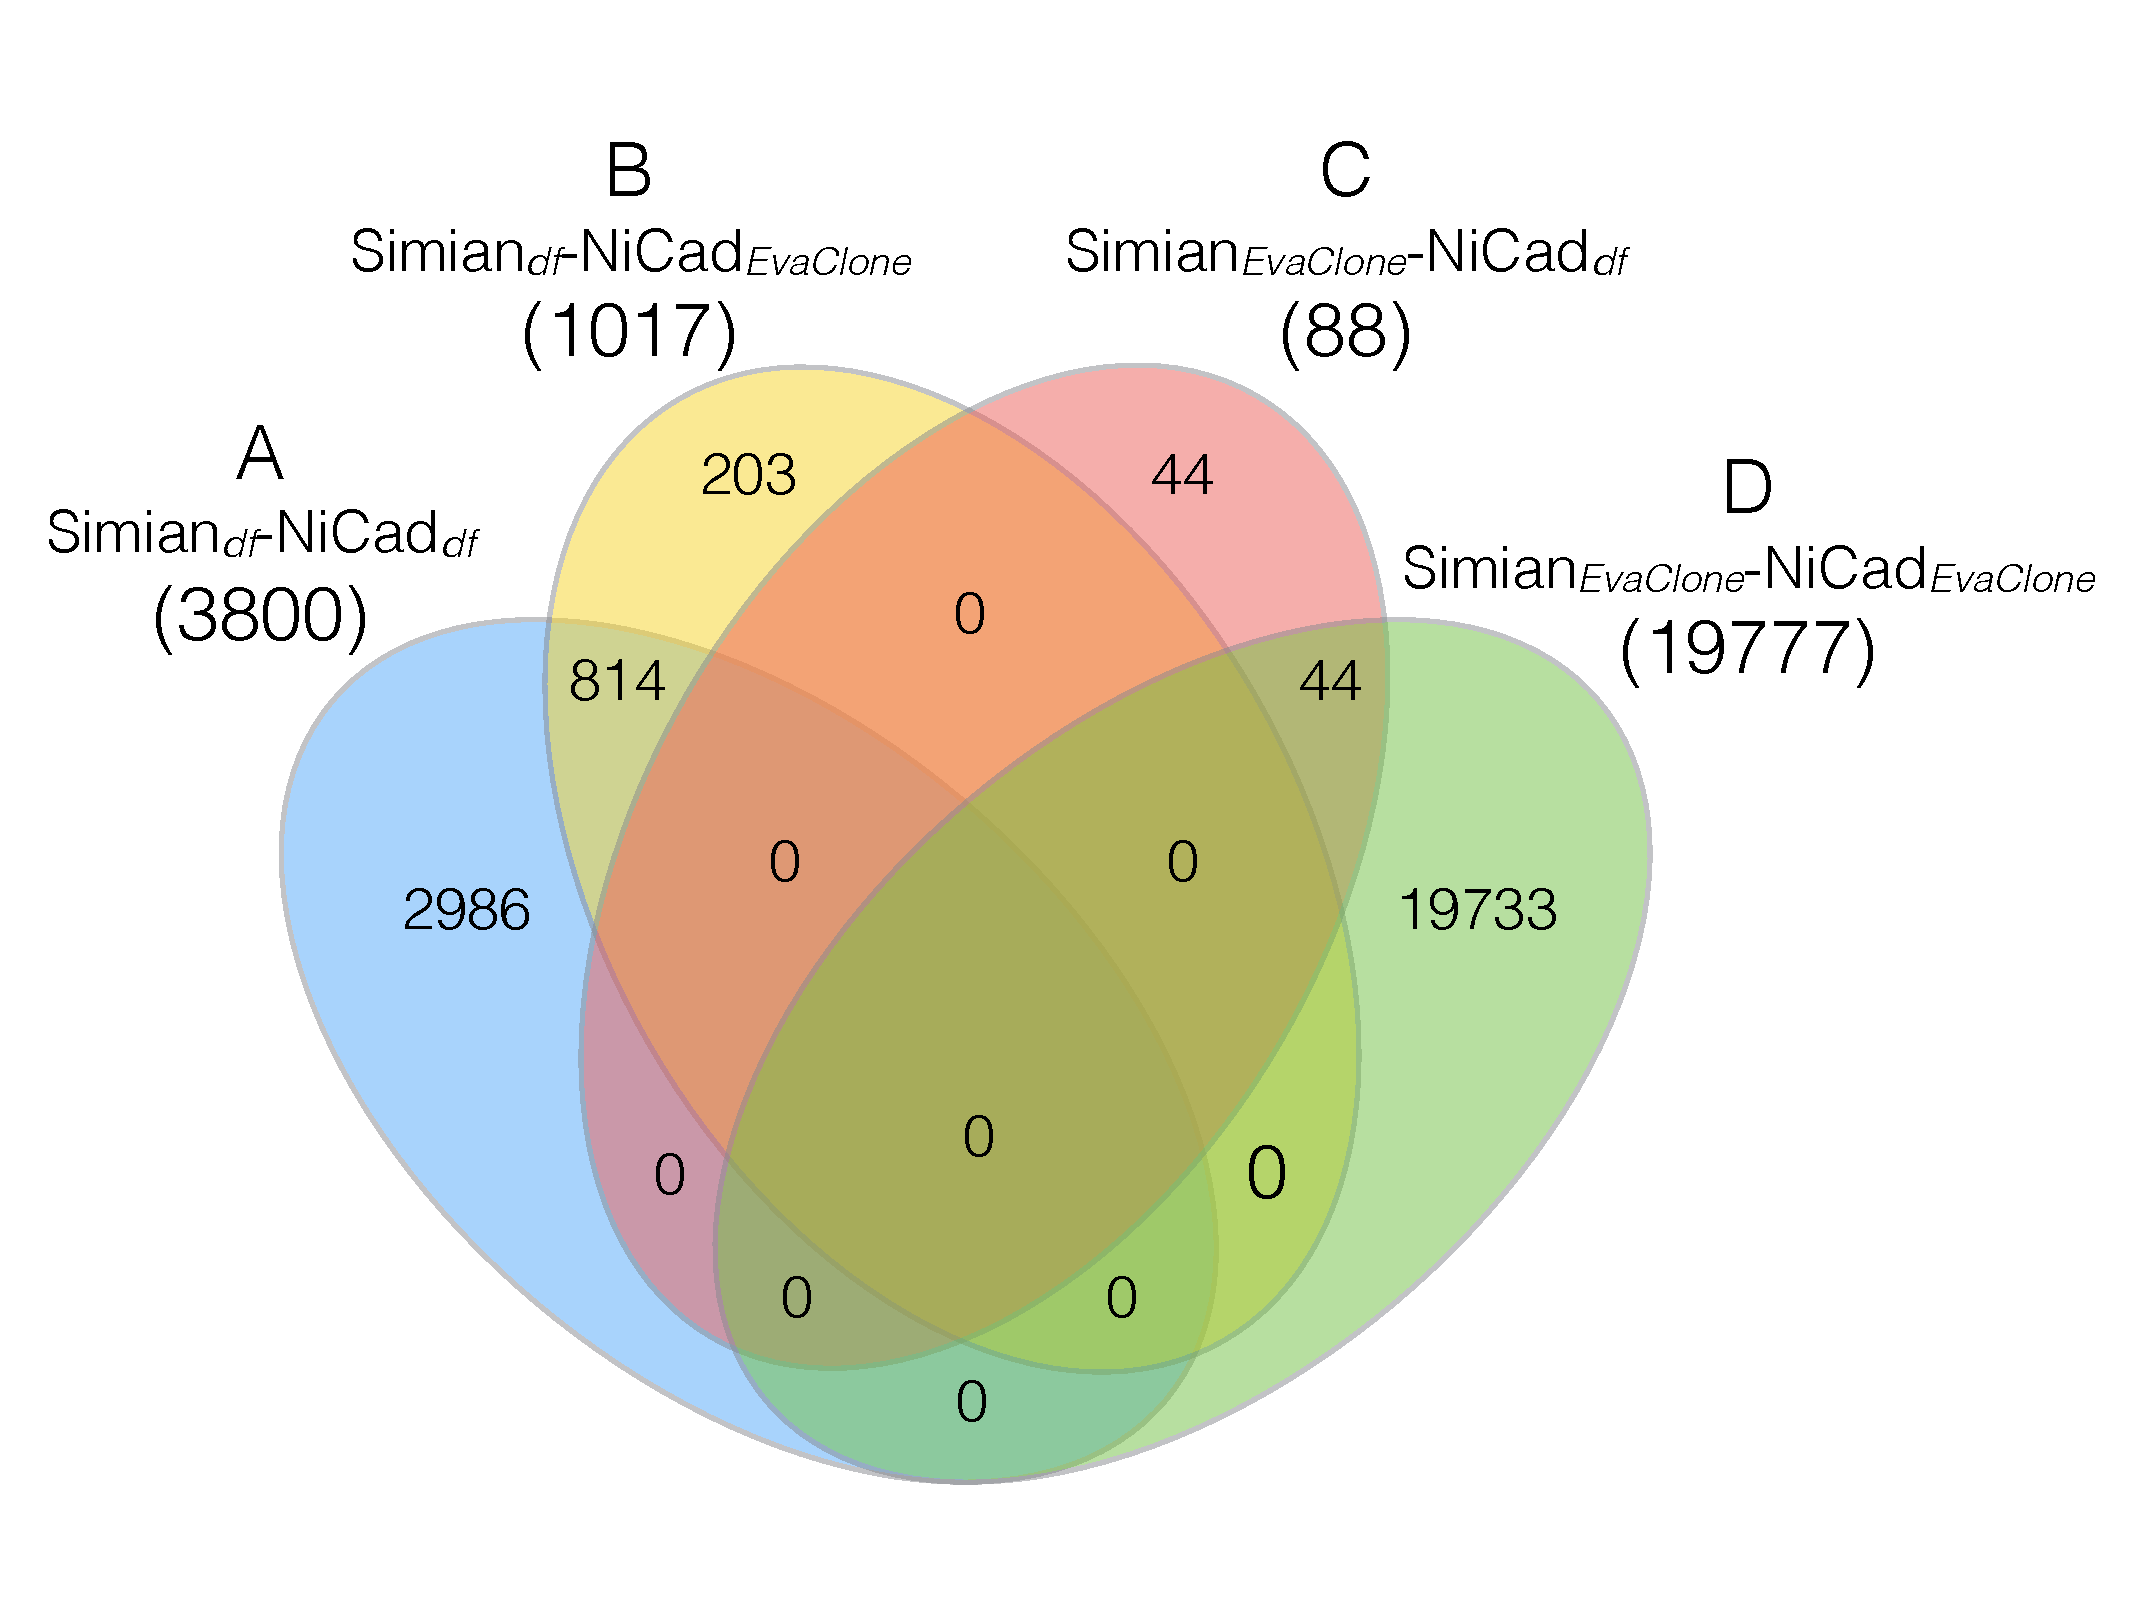
\includegraphics[width=0.8\linewidth]{venn4_pairs_ok_pt1+2}
		\caption{Distributions of \textit{ok}-match(0.7) pairs}
		\label{fig:venn4_orig_ok}
	\end{minipage}
\end{figure*}

\subsubsection{Manual investigation of agreement-based clone pairs}

\begin{table*}
	\centering
	\caption{Classifications of clone creation}
	\label{tab:classification_scheme}
	\begin{tabular}{|c|p{13cm}|}
		\hline 
		Category & Descriptions \\ 
		\hline 
		A & Code in Stack Overflow is copied from Qualitas (Q $\rightarrow$ S). \\ 
		\hline 
		A' & Code in Qualitas is copied from Stack Overflow (S $\rightarrow$ Q). \\ 
		\hline 
		B & Clone pair is exactly identical or highly similar and may be copied either from each other or a third source (unknown) (S $\leftrightarrow$ Q $\vee$ (T $\rightarrow$ S $\wedge$ T $\rightarrow$ Q)).
		\\ 
		\hline 
		C & Code in both places are copied from a third source T (known) (T $\rightarrow$ S $\wedge$ T $\rightarrow$ Q).
		\\ 
		\hline 
		D & Code is a boiler-plate or IDE auto-generated.
		\\ 
		\hline 
		E & Code in both places initialise a similar/the same object; extend the same class/its subclass; implement the same interface.
		\\ 
		\hline 
		F & Accidental similarity, false clone \\ 
		\hline 
	\end{tabular} 
\end{table*}

The classification scheme is described in \Cref{tab:classification_scheme} and the classification results are shown in \Cref{tab:classification_good_o}. We have manually investigated all of the 2,261 \textit{good-match} ones reported by agreement of four different Simian and NiCad settings.  However, for the \textit{ok-match}, we could not investigate all of the 23,868 pairs manually.  According to the manual investigation of \textit{good-match} results, we found that Simian$_{\textrm{\textit{EvCl}}}$--NiCad$_{\textrm{\textit{EvCl}}}$ produces a large number, 2225 (99.87\%), of false positive results (category D, E, and F). Thus, we decided to leave them out of the manual investigation of \textit{ok-match} pairs. There are totally 608 \textit{ok-match} pairs that were investigated. The 39 true positive pairs found are combinations of 8 unique Stack Overflow fragments, and 9 unique Qualitas Java files from 6 different projects.

Since we are not certain about the direction of copying in the B-classified pairs, we checked the modification time of each Java file in Qualitas project and compare it to the timestamp of Stack Overflow answers. We found that all Stack Overflow code fragments were posted after their respectively similar Java files in Qualitas project. This means that the copying can only be either (1) Q $\rightarrow$ S or (2) from a third source to both S and Q independently.

%\textbf{Qualitas-\textbf{N}:} We decided to filter out the agreed clone pairs reported by agreement of Simian$_{\mathrm{\textit{EvaClone}}}$-NiCad$_{\mathrm{\textit{EvaClone}}}$ altogether due to its large number of false positive. With the remaining 3 agreements, we did manual investigation of agreed \textit{ok}-match clone pairs from agreements of Simian$_{df}$-NiCad$_{df}$, Simian$_{df}$-NiCad$_{\mathrm{\textit{EvaClone}}}$, and Simian$_{\mathrm{\textit{EvaClone}}}$-NiCad$_{df}$. We had not done any investigation of \textit{good}-match since there were no \textit{good}-match pairs for these 3 agreements. The number of pairs that have been looked at is 6,706 (excluding duplicates). The results are shown in Table.

\begin{table*}
	\centering
	\caption{Classification results of agreement-based and non agreement-based clone pairs)}
	\label{tab:classification_good_o}
	\small
	\resizebox{2.1\columnwidth}{!}{%
	\begin{tabular}{|l"r|r|r|r|r|r|r|r"r|r|r|r|r|r|r"r|r|r|r|}
		\hline
		Classificaiton & A & A' & B & C & \textbf{Sum} & S$_{u}$ & Q$_u$ & Q$_{up}$ & D  & E & F & \textbf{Sum} & S$_{u}$ & Q$_u$ & Q$_{up}$ & \textbf{Total}  & S$_{u}$ & Q$_u$ & Q$_{up}$\\ 
		\hline 
		\hline
		\multirow{1}{*}{\textit{good-match(0.7)}}  & 1 & 0 & 4  & 3 & \textbf{8} & 7 & 6 & 6 & 58  & 6 & 2189 & \textbf{2253} & 81 & 693 & 58 & \textbf{2261} & 87 & 699 & 59 \\
		\multirow{1}{*}{\textit{ok-match(0.7)}}  & 8 & 0 & 33  & 8 & \textbf{49} & 12 & 14 & 10 & 4459 & 35 & 82 & \textbf{4576} & 99 & 136 & 29 & \textbf{4625} & 110 & 150 & 33 \\
		\hline 
		\hline 
		%		\multirow{1}{*}{\textit{Simian$_{df}$}} & 35 & 0 & 90 & 8 & \textbf{133} & 68 & 59 & 23 & 13 & 12 & 134 & \textbf{159} & 39 & 72 & 23 & \textbf{292} & 103 & 125 & 31 \\
		%		\multirow{1}{*}{\textit{Simian$_{df}$}} & 36 & 0 & 229 & 3 & \textbf{268} & 76 & 151 & 14 & 169 & 52 & 14 & \textbf{235} & 92 & 119 & 22 & \textbf{503} & 164 & 261 & 24 \\
		\multirow{1}{*}{\textit{Simian$_{df}$}} & 71 & 0 & 319 & 11 & \textbf{401} & 138 & 210 & 37 & 182 & 64 & 148 & \textbf{394} & 120 & 191 & 45 & \textbf{795} & 246 & 386 & 55 \\
		\hline
		%		\multirow{1}{*}{\textit{NiCad$_{df}$}} & 4  & 0 & 5 & 0 & \textbf{9} & 9 & 5 & 4 & 24 & 3 & 78 & \textbf{105} & 41 & 39 & 12 & \textbf{114} & 48 & 44 & 14 \\ 
		%		\multirow{1}{*}{\textit{NiCad$_{df}$}} & 0  & 0 & 10 & 0 & \textbf{10} & 7 & 8 & 5 & 6 & 3 & 26 & \textbf{35} & 17 & 16 & 8 & \textbf{45} & 24 & 24 & 9 \\ 
		\multirow{1}{*}{\textit{NiCad$_{df}$}} & 4  & 0 & 15 & 0 & \textbf{19} & 15 & 13 & 9 & 30 & 6 & 104 & \textbf{140} & 51 & 55 & 20 & \textbf{159} & 66 & 68 & 23 \\ 
		\hline
		%		\multirow{1}{*}{\textit{NiCad$_{df}$}*} & 4  & 0 & 1 & 0 & \textbf{5} & 4 & 5 & 3 & 23 & 1 & 67 & \textbf{91} & 28 & 31 & 10 & \textbf{96} & 33 & 37 & 13 \\ 
			%		\hline
	\end{tabular} 
	}
\end{table*}

%\begin{table}
%	\centering
%	\caption{Distribution of classification category A--F according to \textit{good}- and \textit{ok-}match pairs. S denotes Simian and N denotes NiCad tool.}
%	\label{tab:good_classification}
%	\small
%	\begin{tabular}{|l|r|r|r|r|r|r|r|r|}
%		\hline 
%		Category   & A   & 	A'   & 	B   & C   & D   &	E   &	F   & Total  \\
%		\hline
%		\hline
%		\multicolumn{9}{|c|}{\textit{good}-match pairs} \\
%		\hline
%		S$_{df}$--N$_{df}$   & 1 & 0 & 1 & 0 & 1 & 4 & 0 & 7 \\
%		S$_{df}$--N$_{\textrm{\textit{EvCl}}}$   & 1 & 0 & 0 & 3 & 14 & 1 & 1 & 20 \\
%		S$_{\textrm{\textit{EvCl}}}$--N$_{df}$   & 0 & 0 & 3 & 0 & 7 & 0 & 0 & 10 \\
%		S$_{\textrm{\textit{EvCl}}}$--N$_{\textrm{\textit{EvCl}}}$   & 0 & 0 & 1 & 0 & 20 & 0 & 2188 & 2228 \\
%		\hline
%		Total   &   2   &   0   &  2   &  6   &   26   &   10   & 1320  & 1366 \\
%		Total (unique)  &   1   &   0   &  1   &  3   &   26   &   6   & 1320  & 1352 \\
%		\hline
%		\hline 
%%		Category   																										& A   	& 	A' 	& 	B  & C	   & D   	&	E   &	F   & Total  \\
%%		\hline
%		\multicolumn{9}{|c|}{\textit{ok}-match pairs} \\
%		\hline
%		S$_{df}$--N$_{df}$        & 3 	& 0 	& 12	& 6 	& 3755  & 8	& 7  &  3791 \\
%		S$_{df}$--N$_{\textrm{\textit{EvCl}}}$   	& 8 	& 0 	& 28	& 4	& 904 & 29  & 32 &  1005 \\
%		S$_{\textrm{\textit{EvCl}}}$--N$_{df}$   	& 0 	& 0 	& 0 	& 0 	 & 29 	  & 0 		& 24 	& 53 \\
%		\hline
%		Total   &   11  &   0   &  32   &  10   &   712   &   30   & 63  & 858 \\
%		Total (unique)  &   8  &   0   &  23   &  8   &  480  &  28  & 61  & 608 \\
%		\hline
%	\end{tabular} 
%\end{table}

\subsection{Non-agreement based clone pairs}
In the preliminary stage of our experiment, we found that there are 41 Stack Overflow fragments reported by Simian with default configurations. However, only 10 of them appear in the new results using tool's agreement. Thus, we further investigated the clone pairs reported by Simian and NiCad but \textit{without} an agreement. 

With our 4 settings, we decided to investigate only 2 settings, Simian$_{df}$, and NiCad$_{df}$, and drop Simian$_{\mathrm{\textit{EvaClone}}}$ and NiCad$_{\mathrm{\textit{EvaClone}}}$ due to their large number of false positives as shown in \Cref{tab:good_classification} and \Cref{tab:ok_classification}. With the 2 selected settings, we investigated clone pairs having the minimum clone size of 10 SLOC as they are meaningful and tend to be real clone in modern clone detection \cite{Sajnani2016}. 

For Simian$_{df}$, there were 9,383 clone pairs reported by the tool. Out of 9,383 pairs, 140 of them are the ones found in \textit{ok-}pairs using agreement-based detection. We filtered the results further by removing false positives such as similar equals(), hashCode() methods, getters and setters out by using regular expression. We managed to remove 8,956 pairs using this method. Eventually, there were 287 clone pairs remaining for manual investigation. For NiCad$_{df}$, we obtained 7,040 clone pairs to look at which is infeasible for manual investigation. Hence, result filtering was also needed. However, regular expressions could not be used effectively as in Simian's case since NiCad allowed clones that are different at keywords/variable names or even added/deleted lines. So we decided to filter the results by selecting pairs that pass stricter clone criteria with $\mathrm{UPI} = 0.2$. By reducing the UPI to 0.2, there were totally 166 pairs left. Out of 166, 52 are \textit{ok}-pairs and 114 are remaining pairs for manual check (18 pairs are from \textit{cayenne} and \textit{iReport} that could not be analysed using UPI = 0.3). The statistics of the clones and classification results are reported in \Cref{tab:classification_indv_stats}.

%We selected only Stack Overflow fragment and Qualitas files that have never been looked at before in the previous investigation. If many clone pairs having the same Stack Overflow fragment and Qualitas file, we keep only the largest one. The reason for having this criteria is that we found a lot of duplicate clone pairs with the same classifications from either Stack Overflow fragments or Qualitas files. The classification results are shown in Table \ref{tab:classification_indv}. 

\begin{table}
	\centering
	\caption{Statistics of non agreement-based clone pairs (Simian$_{df}$ and NiCad$_{df}$).}
	\label{tab:classification_indv_stats}
	\small
	\begin{tabular}{l|r|r|r|r}
		\hline 
		Tool & Clone pairs & \textit{ok}-pairs & filtered & remaining \\ 
		%\hline 
		%\multirow{1}{*}{\textit{Simian$_{df}$}-1} & 9383 & 140 & 8951 & 292 \\
		%\multirow{1}{*}{\textit{Simian$_{df}$}-2} & 9042 & 0 & 8539 & 503 \\
		\hline
		\multirow{1}{*}{\textit{Simian$_{df}$}} & 18425 & 140 & 17490 & 795 \\
		\hline
%		\multirow{1}{*}{\textit{NiCad$_{df}$}-1} & 7040  & 226 & 6700 & 114 \\
%		\multirow{1}{*}{\textit{NiCad$_{df}$}-2} & 22187  & 152 & 21990 & 45 \\
		\multirow{1}{*}{\textit{NiCad$_{df}$}} & 29227  & 378 & 28690 & 159 \\
		\hline
	\end{tabular} 
\end{table}

\subsubsection{Manual investigation of non agreement-based clone pairs}
%\subsubsection*{\textbf{Qualitas-\textit{O} (v. 2013-09-01r)}}
We performed manual investigation and classified the clone pairs reported by Simian$_{df}$ and NiCad$_{df}$ in the same way as the agreement-based clone pairs. The results of the manual investigation is reported in \Cref{tab:classification_good_o}.

%\subsection{Summary of true online clone pairs}
\begin{table}[H]
	\centering
	\caption{Numbers of true positive online clone pairs found by manual investigation}
	\label{tab:classification_true_pairs_summary}
	\small
	\begin{tabular}{l|r|r|r|r|r}
		\hline 
		Tool & A & A' & B & C & Total \\
		\hline
		\textit{good}-pairs & 1 & 0 & 4 & 3 & 8 \\
		\textit{ok}-pairs & 8 & 0 & 33 & 8 & 49 \\
%		Simian$_{df}$ pairs-1 & 35 & 0 & 90 & 8 & 133 \\
%		Simian$_{df}$ pairs-2 & 36 & 0 & 229 & 3 & 268 \\
		Simian$_{df}$ pairs & 71 & 0 & 319 & 11 & 401 \\
%		NiCad$_{df}$ pairs & 4 & 0 & 5 & 0 & 9 \\
%		NiCad$_{df}$ pairs-2 & 0 & 0 & 10 & 0 & 10 \\
		NiCad$_{df}$ pairs & 4 & 0 & 15 & 0 & 19 \\
		\hline 
		Total & 84 & 0 & 371 & 22 & 477 \\
		\hline
	\end{tabular} 
\end{table}

\begin{figure}
	\centering
	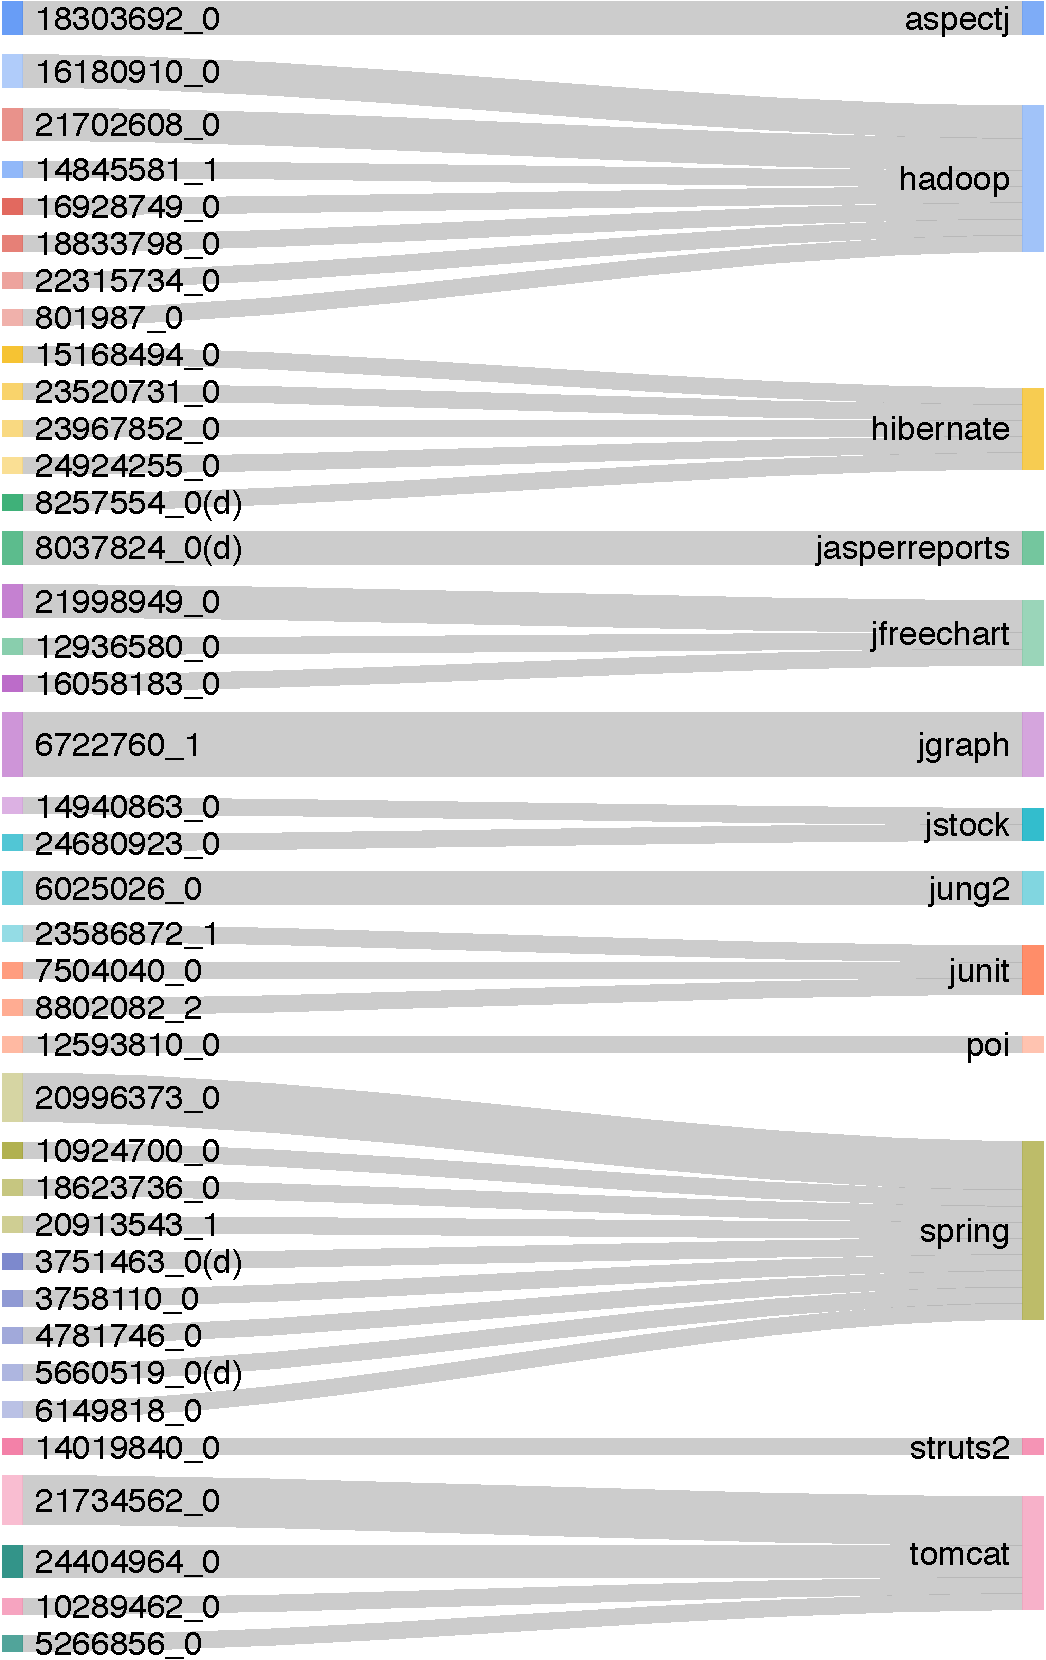
\includegraphics[width=0.8\linewidth]{Sankey_proj}
	\caption{Relationships of 53 Stack Overflow clone pairs to their original projects. 49 are outdated and 4 are deleted (shown using (d) suffix).}
	\label{fig:sankey}
\end{figure}

%\subsubsection{Qualitas-\textit{N} (v. 2016-08-05)}

\section{Effects of online code clone}

In this study, we are interested in the effects of online code clones to software development. From the manual investigation of 184 true online clone pairs, we found that there are two potential issues: stale online code, and software licensing violation.

\subsection{Issue~1 -- stale online code clones}
Stale online code occurs when a piece of code has been copied from a software project to Stack Overflow, and later it has been changed in the original project. However, in this situation, the copy is still unchanged. Since the code were updated due to various possible reasons including bug fixing, this can cause a problem if developers reuse stale online code from Stack Overflow. They might also introduce the same unfixed bug(s) into the software. To discover stale online code, we focus on the true online clone pairs that are copied in the direction from Qualitas to Stack Overflow (category-\textit{A} online clone pairs) in \Cref{tab:classification_true_pairs_summary} which results in 84 pairs selected. %We restricted it further to only the ones having versioning system so we can trace changes made to these clone pairs. Fortunately, all of the pairs were from projects with either git or svn so we did not remove any pair from this set. 

%Our intuition behind his issue comes from a situation where a piece of code has been copied from a Qualitas project and posted on Stack Overflow. Later, that piece of code has been modified further to accommodate changes in the projects (or any other reasons). However, even the code in Qualitas project is already updated, the one posted on Stack Overflow is not changed. This results in outdated online code which can cause problems when programmers copy and use it in their projects.

%We decided to ignore NiCad results from this analysis due to its failure of clone clustering and renaming on some projects.  Thus, the 39 projects are the ones that can be analysed by Simian, have newer versions than the versions in Qualitas-\textit{O}, and have code version control system (either git or svn). %After filtering, there are 141 pairs removed because 45 of them do not have new versions (7 from c-jdbc, 21 from Compiere, 7 from heritrix, and 10 from iReport) and 4 of them we could not find source code with version control (2 from findbugs, 1 from jag, and 1 from jgraphpad). Finally there were 134  pairs remaining. %We are interested in clone pairs that were changed after they appeared on Stack Overflow.

\Cref{tab:stale_code} shows the results of manual investigation of 84 category-A online clone pairs. The investigation reveals that there are 50 clone pairs that are outdate (i.e. ``stale clone''). They are clone pairs that were copied from Qualitas projects to Stack Overflow and marked as accepted answers, and later have been changed during the development.  

\begin{table}
	\centering
	\caption{Results from a manual investigation of 84 category-A online clone pairs}
	\label{tab:stale_code}
	\small
%	\resizebox{\columnwidth}{!}{%
	\begin{tabular}{l|r|r|r|r|r}
		\hline 
		Project & Pairs & Stale & Fresh & Del. & Others \\
		\hline
		ant & 1 & 0 & 1 & 0 & 0 \\
		log4j & 4 & 0 & 4 & 0 & 0 \\
		tomcat & 7 & 7 & 0 & 0 & 0 \\
		aspectj & 2 & 2 & 0 & 0 & 0 \\
		hadoop & 14 & 9 & 5 & 0 & 0 \\
		hibernate & 16 & 4 & 11 & 1 & 0 \\
		jasperreports & 2 & 2 & 0 & 0 & 0 \\
		jfreechart & 4 & 4 & 0 & 0 & 0 \\
		jgraph & 5 & 4 & 0 & 0 & 1 \\
		jgrapht & 1 & 0 & 1 & 0 & 0 \\
		jstock & 2 &  2 & 0 & 0 & 0 \\
		jung & 2 & 2 & 0 & 0 & 0 \\
		junit & 3 & 3 & 0 & 0 & 0 \\
		poi & 3 & 1 & 2 & 0 & 0 \\
		spring & 14 & 9 & 3 & 2 & 0 \\
		struts & 1 & 1 & 0 & 0 & 0 \\
		weka & 3 & 0 & 3 & 0 & 0 \\
		\hline
		Total & 84 & 50 & 30 & 3 & 1 \\
		\hline
	\end{tabular} 
%}
\end{table}

\begin{table*}
	\centering
	\caption{53 code clones in Stack Overflow that were altered, rewritten, or removed from the project after posted}
	\label{tab:stale_code_details}
	\small
	\begin{tabular}{r|l|l|r|c|l}
		\hline 
		No. & Project & File & SO Post & Changes & Date \\
		\hline
		1 &  aspectj-1.6.9  &  Agent.java  & 18303692 &  alteration  & 2015-09-08 \\
		2 &  aspectj-1.6.9   &  Agent.java  & 18303692 &  alteration  & 2015-09-08 \\
		3 &  hadoop-1.0.0  &  DBCountPageView.java  & 21702608 &  alteration & 2011-06-12 \\
		4 &  hadoop-1.0.0  &  DBCountPageView.java  & 21702608 &  alteration  & 2011-06-12 \\
		5 &  hadoop-1.0.0  &  JobSubmissionFiles.java  & 14845581 &  alteration  & 2012-06-25 \\
		6 &  hadoop-1.0.0  &  LineRecordReader.java  & 16180910 &  alteration & 2011-07-25 \\
		7 &  hadoop-1.0.0  &  LineRecordReader.java  & 16180910 &  alteration  & 2011-07-25 \\
		8 &  hadoop-1.0.0  &  StringUtils.java  & 801987 &  alteration & 2013-02-04 \\
		9 &  hadoop-1.0.0  &  TestJobCounters.java  & 18833798 &  alteration  & 2011-06-12 \\
		10 &  hadoop-1.0.0  &  TextOutputFormat.java  & 16928749 &  alteration  & 2011-06-12 \\
		11 &  hadoop-1.0.0  &  WritableComparator.java  & 22315734 &  alteration & 2014-11-20 \\
		12 &  hibernate-4.2.2  &  ConnectionProviderInitiator.java  & 15168494 &  alteration  & 2012-06-24 \\
		13 &  hibernate-4.2.2  &  Example.java  & 24924255 &  alteration  & 2013-04-23 \\
		14 &  hibernate-4.2.2  &  SchemaUpdate.java  & 23520731 &  alteration & 2016-02-05 \\
		15 &  hibernate-4.2.2  &  SettingsFactory.java  & 8257554 &  removal & 2011-03-11 \\
		16 &  hibernate-4.2.2  &  SQLServer2005LimitHandler.java  & 23967852 &  alteration  & 2015-03-12 \\
		17 &  jasperreports-3.7.4  &  JRVerifier.java  & 8037824 &  alteration  & 2008-04-17 \\
		18 &  jasperreports-3.7.4  &  JRVerifier.java  & 8037824 &  alteration & 2011-05-20 \\
		19 &  jfreechart-1.0.13  &  AbstractXYItemRenderer.java  & 12936580 &  alteration  & 2016-02-19 \\
		20 &  jfreechart-1.0.13  &  KeyToGroupMap.java  & 16058183 &  alteration  & 2013-07-03 \\
		21 &  jfreechart-1.0.13  &  SpiderWebPlot.java  & 21998949 &  alteration  & 2008-06-02 \\
		22 &  jfreechart-1.0.13  &  SpiderWebPlot.java  & 21998949 &  alteration  & 2008-06-02 \\
		23 &  jgraph-5.13.0.0  &  HelloWorld.java  & 6722760 &  rewriting  & 2014-04-13 \\
		24 &  jgraph-5.13.0.0  &  HelloWorld.java  & 6722760 &  rewriting  & 2014-04-13 \\
		25 &  jgraph-5.13.0.0  &  HelloWorld.java  & 6722760 &  rewriting  & 2014-04-13 \\
		26 &  jgraph-5.13.0.0  &  HelloWorld.java  & 6722760 &  rewriting  & 2014-04-13 \\
		27 &  jstock-1.0.7c  &  GoogleMail.java  & 14940863 &  alteration & 2015-12-13 \\
		28 &  jstock-1.0.7c  &  GoogleMail.java  & 24680923 &  alteration  & 2015-12-13 \\
		29 &  jung2-2\_0\_1  &  ShortestPathDemo.java  & 6025026 &  alteration  & 2010-04-13 \\
		30 &  jung2-2\_0\_1  &  ShortestPathDemo.java  & 6025026 &  alteration  & 2010-04-13 \\
		31 &  junit-4  &  Assert.java  & 23586872 &  alteration  & 2015-05-12 \\
		32 &  junit-4  &  ExternalResource.java  & 7504040 &  alteration & 2016-06-25 \\
		33 &  junit-4.11  &  ExpectException.java  & 8802082 &  alteration & 2014-05-26 \\
		34 &  poi-3.6-20091214  &  WorkbookFactory.java  & 12593810 &  alteration  & 2015-04-29 \\
		35 &  spring-framework-3.0.5  &  AnnotationMethodHandlerExceptionResolver.java  & 5660519 &  removal & 2012-01-20 \\
		36 &  spring-framework-3.0.5  &  AutowireUtils.java  & 20913543 &  alteration  & 2014-10-28 \\
		37 &  spring-framework-3.0.5  &  CustomCollectionEditor.java  & 18623736 &  alteration  & 2013-11-21 \\
		38 &  spring-framework-3.0.5  &  DefaultAnnotationHandlerMapping.java  & 3758110 &  removal  & 2012-01-20 \\
		39 &  spring-framework-3.0.5  &  DefaultPropertiesPersister.java  & 6149818 &  alteration  & 2013-03-19 \\
		40 &  spring-framework-3.0.5  &  DelegatingServletInputStream.java  & 20996373 &  alteration  & 2016-07-15 \\
		41 &  spring-framework-3.0.5  &  DelegatingServletInputStream.java  & 20996373 &  alteration  & 2008-12-18 \\
		42 &  spring-framework-3.0.5  &  DelegatingServletInputStream.java  & 20996373 &  alteration  & 2008-12-18 \\
		43 &  spring-framework-3.0.5  &  DispatcherServlet.java  & 4781746 &  alteration  & 2011-08-08 \\
		44 &  spring-framework-3.0.5  &  Jaxb2Marshaller.java  & 10924700 &  alteration  & 2012-08-28 \\
		45 &  spring-framework-3.0.5  &  ScheduledTasksBeanDefinitionParser.java  & 3751463 &  alteration  & 2016-07-05 \\
		46 &  struts2-2.2.1  &  DefaultActionMapper.java  & 14019840 &  alteration  & 2013-10-18 \\
		47 &  tomcat-7.0.2  &  BasicAuthenticator.java  & 21734562 &  alteration  & 2016-08-04 \\
		48 &  tomcat-7.0.2  &  BasicAuthenticator.java  & 21734562 &  alteration & 2016-08-04 \\
		49 &  tomcat-7.0.2  &  CoyoteAdapter.java  & 24404964 &  alteration  & 2012-11-18 \\
		50 &  tomcat-7.0.2  &  CoyoteAdapter.java  & 24404964 &  alteration  & 2012-11-18 \\
		51 &  tomcat-7.0.2  &  FormAuthenticator.java  & 21734562 &  alteration & 2016-08-04 \\
		52 &  tomcat-7.0.2  &  HttpServlet.java  & 5266856 &  alteration  & 2011-10-22 \\
		53 &  tomcat-7.0.2  &  JspRuntimeLibrary.java  & 10289462 &  alteration  & 2012-09-12 \\
		\hline
	\end{tabular} 
\end{table*}

\subsection{Issue~2 -- software licensing violations}
Software licensing is a paramount factor in software development. Violation of software license can cause a major impact to the delivery of the software and also lead to legal issues. It is an emerging area that software engineering research community is paying attention to. For example, there are studies of automatic technique to identify software licensing from source code files \cite{German2010} and the evolution of licenses in open source projects \cite{DiPenta2010}.

In our study, we reveal another possible situation of software licensing issue caused by code cloning to Stack Overflow. We found that there are at least 84 pieces of code have been copied from 13 open source projects in Qualitas dataset to Stack Overflow as examples. They are also marked as accepted answers which increase their probability of being reused. These 13 open source projects come with their respective software licenses. However, the licensing information are mostly missing from these clones when they are posted on Stack Overflow. Mostly one or a few methods from the full source file are cloned. This makes the license information at the top of the file mostly left uncopied. If developers copy and reuse these pieces of code in their projects, a licensing conflict can quietly happen without realisation of the developers. 

%\section{Investigation of Missing A/B Clone Pairs Reported by Simian$_{df}$}
%We investigated the 41 clone pairs previously reported by Simian with default configurations and manually investigated. The 41 pairs were searched for in 4 new results sets: Simian$_{df}$, Simian$_{\mathrm{\textit{EvaClone}}}$, NiCad$_{df}$, NiCad$_{\mathrm{\textit{EvaClone}}}$. The investigation results are shown in Table \ref{tab:search}.
%
%\begin{table}
%	\centering
%	\caption{Results of matching the original 41 Simian(default) pairs in the pretty-printed result sets}
%	\label{tab:search}
%	\begin{tabular}{l|r|r}
%		\hline 
%		Settings & Found & Not found \\ 
%		\hline 
%		Simian$_{df}$  &  40 & 1* \\ 
%		\hline 
%		Simian$_{\mathrm{\textit{EvaClone}}}$ & 0 & 41  \\ 
%		\hline 
%		NiCad$_{df}$  & 17 & 24 \\ 
%		\hline 
%		NiCad$_{\mathrm{\textit{EvaClone}}}$ &  24 & 17 \\ 
%		\hline 
%	\end{tabular} 
%\end{table}
%
%The single missing Stack Overflow fragment (19051537\_0.java) (denoted by *) is one of the 11 false clones generated by Simian. It is removed from the results of the pretty-printed version because it is an outlier. The rest are missing because of different parameter settings.
%
%\section{Simian's Parameters}
%
%We have carefully investigated the effects of the Simian's parameter \texttt{-balanceSquareBrackets+}. I found that it works in the expected way of handling a pair of brackets (\texttt{[},\texttt{]}) that span over multiple lines. For example, the two code fragments in Figure \ref{fig:two_frags} would match by having \texttt{-balanceSquareBrackets+} enabled. However, the \texttt{-balanceSquareBrackets+} parameter only works on a small testing environment having toy programs or only small pairs from the full datasets. It does not work with the full complete set of 144,075 Stack Overflow fragments and Qualitas projects. Please find the summary of all the testing scenarios in Table \ref{tab:summary}. %I found that this pair is missing if I turned on \texttt{-balanceSquareBrackets+}.
%
%\noindent\begin{figure*}
%	\scriptsize
%	\begin{lstlisting}[frame=single,style=base]
%	1   public class MagicSquare {                           public class MagicSquare2 {
%	2       private int[][] square;                              @private int[@
%	3       private boolean[] possible;                                      @][@
%	4       private int totalSqs;                                            @] square;@
%	5       private int sum;                                     private boolean[] possible;
%	6       private int numsquares;                              private int totalSqs;
%	7       public static void main ( String[] args ) {          private int sum;
%	8       MagicSquare m = new MagicSquare ( 3 );               private int numsquares;
%	9                                                            public static void main ( String[] args ) {
%	10                                                           MagicSquare m = new MagicSquare ( 3 );
%	\end{lstlisting}
%	\caption{Two identical fragments with only differences in locations of the square brackets. All 7 lines are reported by Simian if \small\texttt{-balanceSquareBrackets+} \normalsize is enabled. If not, the clone pairs is reported as \newline (MagicSquare.java [3,8], MagicSquare2.java [5,10]).} 
%	\label{fig:two_frags}
%\end{figure*}
%
%\begin{table*}
%	\caption{Simian's \texttt{-balanceSquareBrackets+} (\texttt{-bsb+}) is observed to have unpredictable behaviours when running against big datasets. $\textrm{\textit{CP}}_2$ means the reported clone(s) do not contain lines having dislocated brackets ($L_b$) (i.e. $\textrm{\textit{CP}}_2 = \textrm{\textit{CP}}_1 - L_b$).}
%	\label{tab:summary}
%	\centering
%	\small\begin{tabular}{l|p{6cm}|c|c|c}
%		\hline 
%		\multirow{2}{*}{\textbf{Project 1}} & \multirow{2}{*}{\textbf{Project 2}} & \textbf{Dislocated} & \multirow{2}{*}{\textbf{-bsb+}} & \textbf{Clones pair} \\ 
%		& & \textbf{brackets?} & & \textbf{reported} \\
%		\hline
%		\hline
%		\multicolumn{5}{l}{\textit{Only run Simian against the pair}} \\
%		\hline
%		MagicSquare.java & MagicSquare\_exact\_copy.java & no & 0,1 & $\textrm{\textit{CP}}_1$ \\
%		MagicSquare.java & MagicSquare2.java & yes & 0 & $\textrm{\textit{CP}}_2$ \\ 
%		MagicSquare.java & MagicSquare2.java & yes & 1 & $\textrm{\textit{CP}}_1$ \\
%		\hline
%		%\hline
%		%\multicolumn{5}{c}{\textit{Only run Simian against the pair}} \\
%		%\hline
%		stackoverflow/4298836\_0.java & Qualitas/aoisrc281/../ExprModule.java & no & 0 & $\textrm{\textit{CP}}_3$ \\ 
%		stackoverflow/4298836\_0.java & Qualitas/aoisrc281/../ExprModule.java & no & 1 & $\textrm{\textit{CP}}_3$ \\ 
%		stackoverflow/4533682\_1.java & Qualitas/cobertura-1/../TouchCollector.java & no & 0 & $\textrm{\textit{CP}}_4$ \\ 
%		stackoverflow/4533682\_1.java & Qualitas/cobertura-1/../TouchCollector.java & no & 1 & $\textrm{\textit{CP}}_4$ \\ 
%		\hline 
%		\hline
%		\multicolumn{5}{l}{\textit{Run Simian against the complete stackoverflow data and the project}} \\
%		\hline
%		stackoverflow/4298836\_0.java & Qualitas/aoisrc281/../ExprModule.java & no & 0 & $\textrm{\textit{CP}}_3$ \\ 
%		\cellcolor{red!10}stackoverflow/4298836\_0.java & \cellcolor{red!10}Qualitas/aoisrc281/../ExprModule.java & \cellcolor{red!10}no & \cellcolor{red!10}1 & \cellcolor{red!10}-- \\ 
%		\hline
%		stackoverflow/4533682\_1.java & Qualitas/cobertura-1/../TouchCollector.java & no & 0 & $\textrm{\textit{CP}}_4$ \\ 
%		\cellcolor{red!10}stackoverflow/4533682\_1.java & \cellcolor{red!10}Qualitas/cobertura-1/../TouchCollector.java & \cellcolor{red!10}no & \cellcolor{red!10}1 & \cellcolor{red!10}-- \\
%		\hline 
%	\end{tabular} 
%\end{table*}

\section{Threats to Validity}

\section{Related Work}
\begin{itemize}
	\item Code clones 
		\begin{itemize}
			\item Definition: Baxter et al. \cite{Baxter1998}
			\item Comparison of clone detectors: \cite{Roy2008, Ragkhitwetsagul2016,Svajlenko2014}
			\item NiCad \cite{Roy2008,Cordy}
			\item Simian \cite{simian}
			\item Clone taxonomy \cite{Kapser2003}
			\item Clone evolution \cite{Pate2013,Mondal2011}
			\item Comparing Quality Metrics for Cloned and non cloned Java Methods : A Large Scale Empirical Study \cite{Saini2016}.
		\end{itemize}
	\item Agreement-based Clone Detection
	\begin{itemize}
		\item Bellon's framework \cite{Bellon2007}.
		\item EvaClone \cite{Wang2013}
		\item Hybrid \cite{Funaro2010}
	\end{itemize}
	\item Software licensing
	\begin{itemize}
		\item Code siblings \cite{German2009}, Ninka -- Automatic indification of SW license \cite{German2010}, Evolution of SW licensing \cite{DiPenta2010}
	\end{itemize}

	\item Stack Overflow
	\begin{itemize}
		\item Code example \cite{Nasehi2012}
		\item Search for code in Stack Overflow \cite{Diamantopoulos2015,Keivanloo2014,Park2014}
	\end{itemize}
\end{itemize}

\section{Conclusions}
This paragraph will end the body of this sample document.
Remember that you might still have Acknowledgments or
Appendices; brief samples of these
follow.  There is still the Bibliography to deal with; and
we will make a disclaimer about that here: with the exception
of the reference to the \LaTeX\ book, the citations in
this paper are to articles which have nothing to
do with the present subject and are used as
examples only.
%\end{document}  % This is where a 'short' article might terminate

%ACKNOWLEDGMENTS are optional
\section{Acknowledgments}
This section is optional; it is a location for you
to acknowledge grants, funding, editing assistance and
what have you.  In the present case, for example, the
authors would like to thank Gerald Murray of ACM for
his help in codifying this \textit{Author's Guide}
and the \textbf{.cls} and \textbf{.tex} files that it describes.

%
% The following two commands are all you need in the
% initial runs of your .tex file to
% produce the bibliography for the citations in your paper.
\bibliographystyle{abbrv}
\bibliography{sigproc}  

\end{document}
